
\section{Training}

We trained the three early exiting models B-\gls{resnet}, B-\gls{densenet} and \gls{msdnet}, along with conventional versions of the \gls{resnet}101 and \gls{densenet}-121. The \gls{dnn}s were trained on the \gls{min100} training set.

In the next section we describe the experimental setup including the training settings. This is followed by describing the results from the training of the models.

\subsection{Experimental Setup}

All code is written in \gls{python} 3.7 \cite{van_rossum_python_1995} using the \gls{pytorch} 1.2
framework \cite{paszke_automatic_2017} and using the \gls{torchvision} 0.4 library \cite{marcel_torchvision_2010}. All code is available at:
{\color{sns-grey}\url{https://github.com/AlexKarlsen/thesis-src}}. 

All training have been accomplished using a \gls{gpu}-workstation equipped with a NVIDIA GeForce 1080 GTX \gls{gpu} using CUDA 10.1 and cuDNN 7.6.3. Trained models are available at: {\color{sns-grey}\url{https://drive.google.com/open?id=1EAl9qGxcm2U3kPhEsHp0HotgNn_LMWa1}} 



\begin{description}
	\item[Number of Epochs] An epoch is a round of training in which every training sample have been presented to the model. All models have been trained for 50 epochs, to fairly compare models the models. Additionally to reduce the training time to allow training multiple models. Training on the available hardware took 30 to 40 hours per model.
	
	\item[Early Stopping] Early stopping is finding the best obtained model by alternating between training and validation phases for each epoch. The best model is the one obtaining the highest accuracy on the validation data. Early stopping is a mechanism to avoid overtraining a model, that then overfits the training data and obtain poor validation accuracy. For \gls{branchynet} we use the model with the highest average accuracy to not favour any part of the model.  
	  
	\item[Optimizer] The weights of \gls{dnn}s are typically trained using a variant of \gls{sgd}. Some more about \gls{sgd} \cite{goodfellow_deep_2016}.
	
	\gls{sgdr} \cite{loshchilov_sgdr:_2016} is a variant of \gls{sgd}, the method have shown faster convergence on a number of datasets, due to its ability to escape local minimas. It follows a cyclic learning rate schedule in contrast to former decaying learning rate schedules. It has shown, in general, to perform better than adaptive optimizers such as Adam \cite{kingma_adam:_2014}, which implement adaptive learnining rate to avoid being stuck in local minimas. 
	
	\gls{sgdr} uses an aggressive cosine annealing schedule with warm restarts. Figure \ref{fig:cosineannealing} illustrates the learning rate schedule.
	
	\begin{figure}
		\centering
		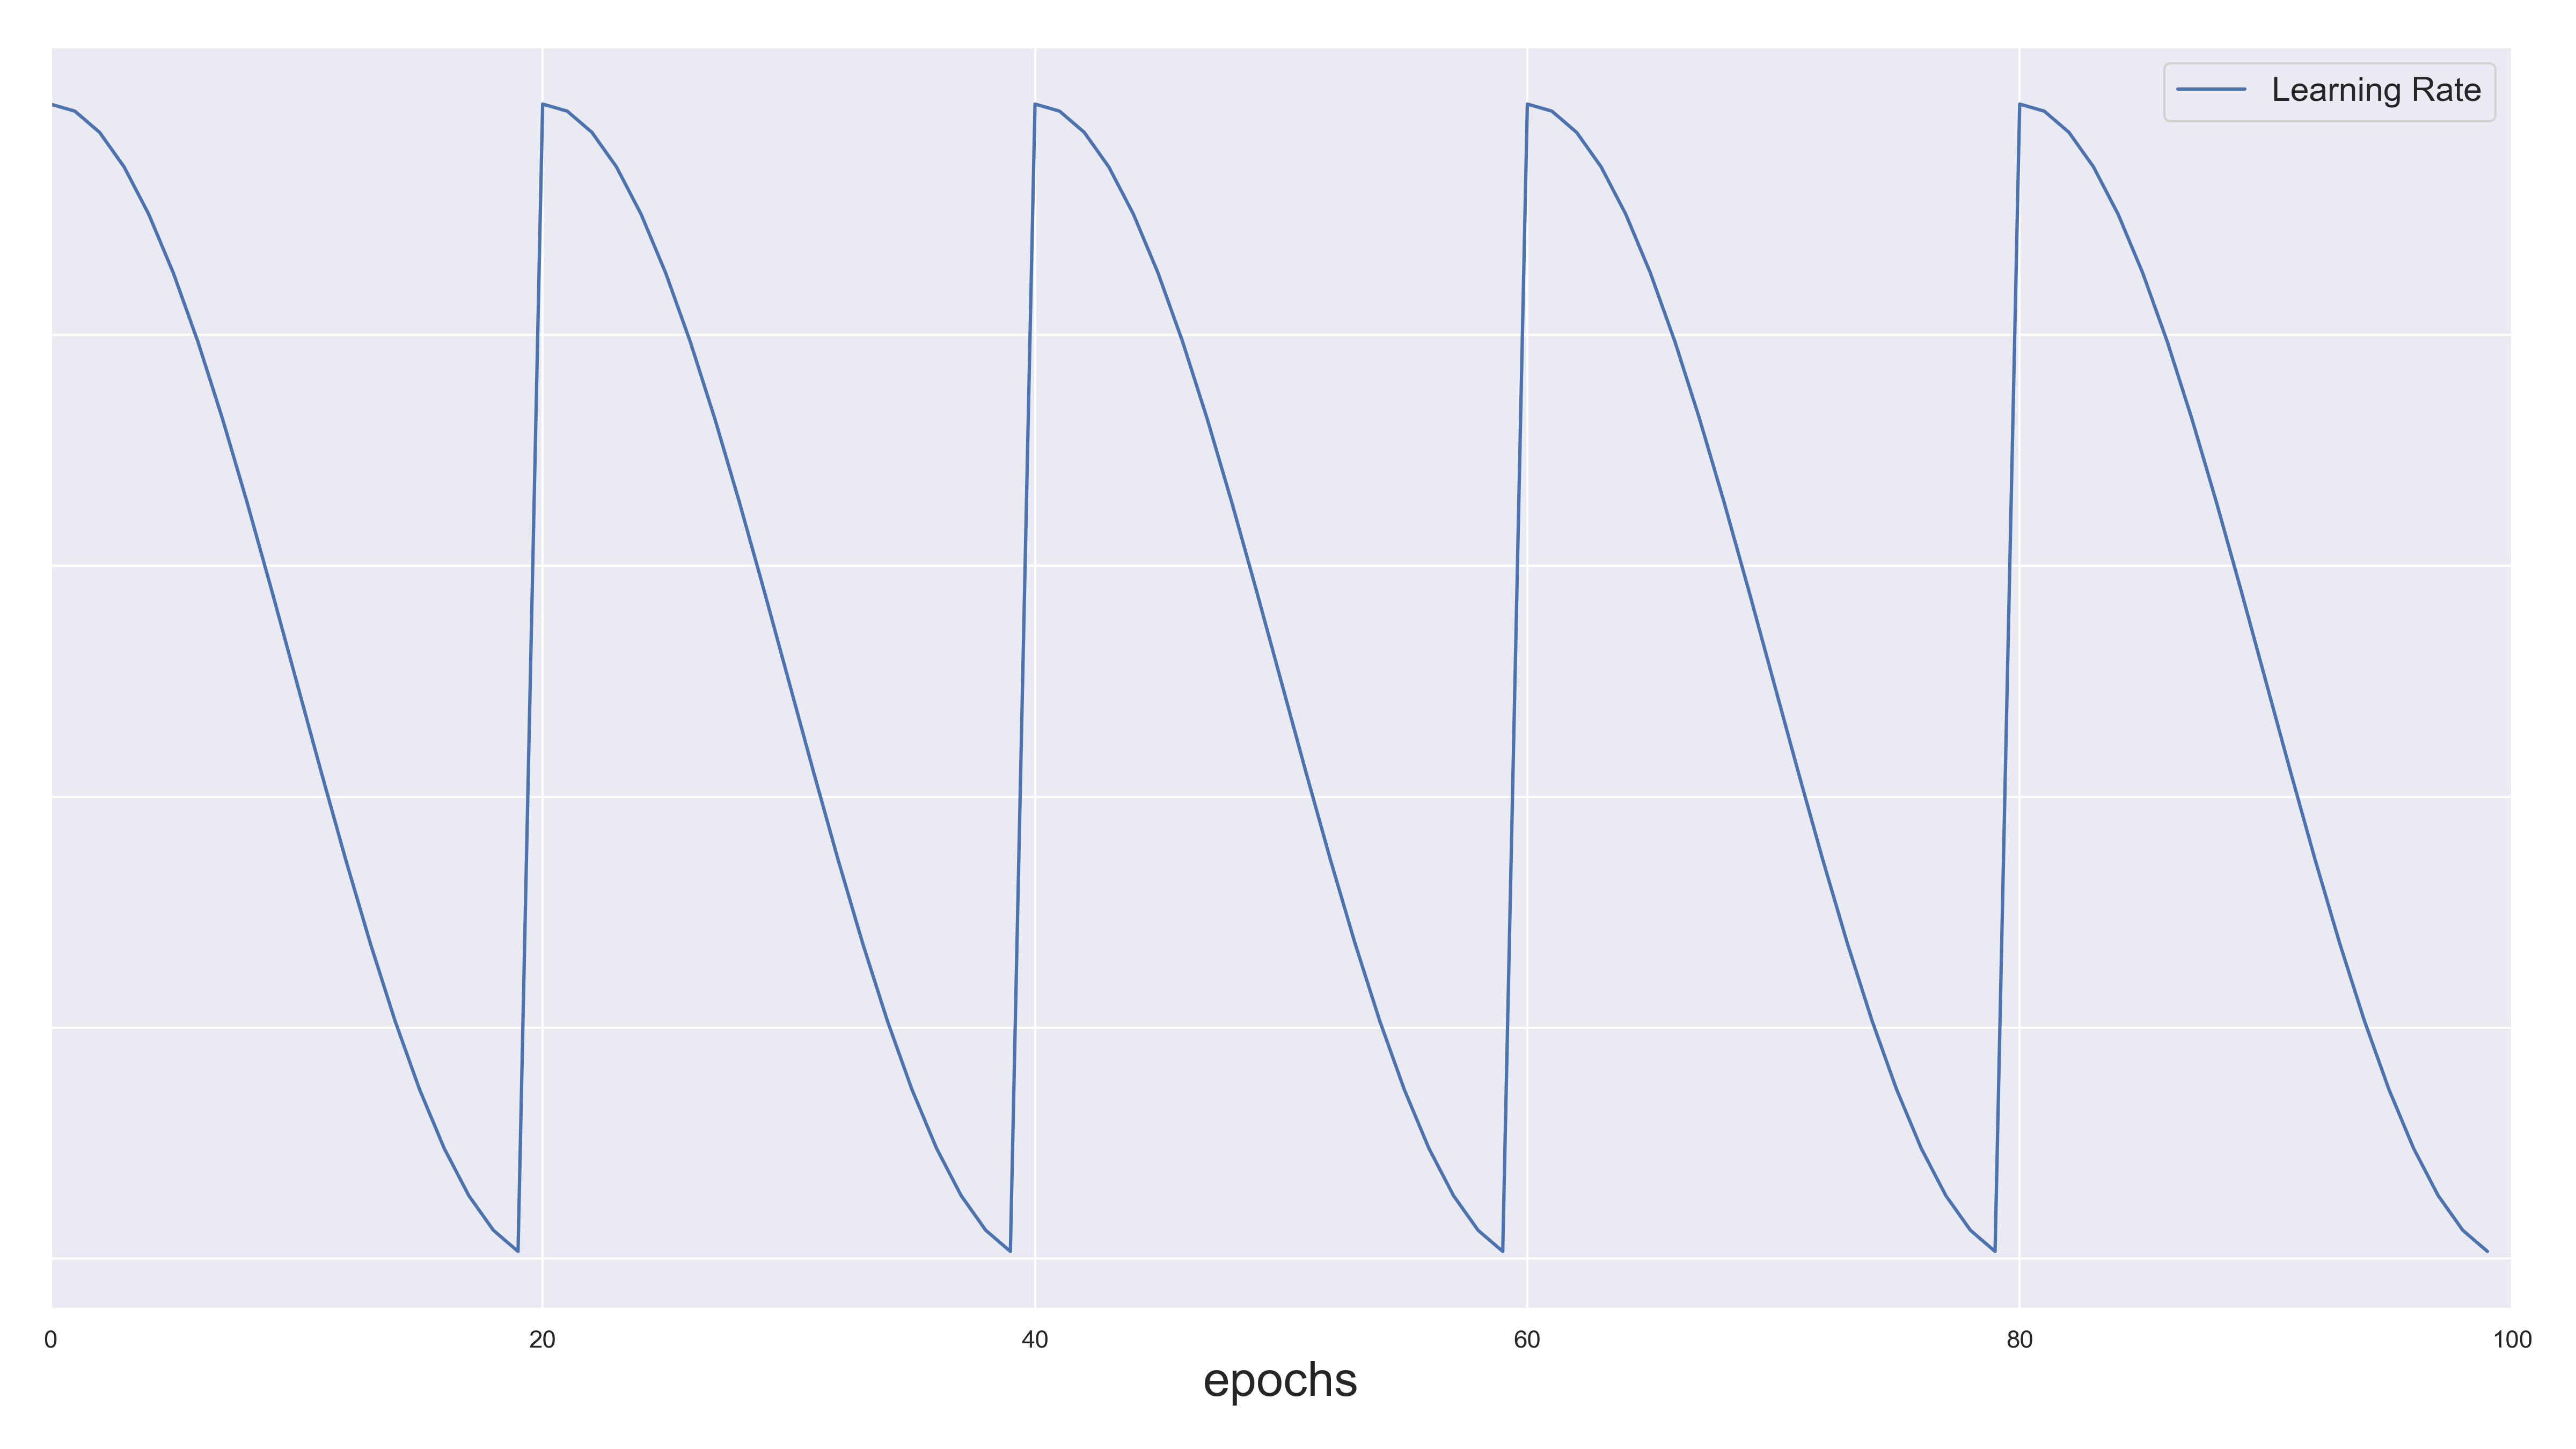
\includegraphics[width=.7\linewidth]{figures/lr.png}
		\caption[Cosine Annealing Learning Rate]{Cosine Annealing Learning Rate} \label{fig:cosineannealing}
	\end{figure}

	\item[Batch Size] Batch Size are recommend to be between 1 and a few hundreds \cite{bengio_practical_2012}, to better utilize \gls{gpu}s a batch size in the power of 2 gives better runtime, e.g. 32 to 256 \cite{goodfellow_deep_2016}. Larger batch sizes have been driving by advancements in parallelism \cite{dean_large_2012}, which can improve the training time, however smaller batch size, have shown better generalization performance due to a regularizing effect \cite{masters_revisiting_nodate}, which especially large model, that tends to overfit can benefit from \cite{goodfellow_deep_2016}. 
	
	In this project a single \gls{gpu} GTX1080 with 8Gb memory is used to train the models. A batch size of 16 is chosen for all \gls{dnn} training sessions, which is the maximum power of 2 possible with the computational budget, as the typical choice of 32 samples in a batch caused memory exhaustion. A batch size of 16 should be adequate and still provide decent training times.
	
	\item[Datasets] \gls{min100} is a subset of the \gls{ilsvrc2012} dataset \cite{russakovsky_imagenet_2015} created for this project, to reduce training time from several weeks to only days on available hardware. The subset is inspired by MiniImageNet \cite{vinyals_matching_2016}, that uses a subset of 100 classes with 600 samples for each class. \gls{min100} contains 100 out of 1.000 randomly sampled classes, which gives 127.300 out of 1.2m training samples and 5.000 out of 50.000 validation samples. A full list of classes are found in the appendix. 
	
	Compared to other sufficiently dense classification datasets e.g \gls{tinyimagenet} \cite{li_cs231n:_2018}, \gls{cifar10} and \gls{cifar100} \cite{krizhevsky_cifar-10_nodate}, the image sizes of these datasets are respectively $(64\times 64$), $(32\times 32)$, $(32\times 32)$ pixels, all of which are considered too small  for this project. Other datasets such as MS COCO and Pascal VOC are better suited for object detection/segmentation, as images are not cropped to only focus on a single object, thus too challenging for classification. In fact Pascal VOC was initially tested, the model however, clearly overfitted the training data due to data sparsity. 
	
	\item[Image Augmentation] A models ability generalize a specific classification problem has a close connection with the number of available training samples. Data augmentation haven proven to be powerful tool in order to virtually create more training data \cite{perez_effectiveness_2017}. Enlarging a training dataset by data augmentation can help create new versions of an image, that are different from but still similar to the original image, without actually having to acquire and annotate new samples \cite{goodfellow_deep_2016}.  
	
	\begin{figure}[H]
		\centering
		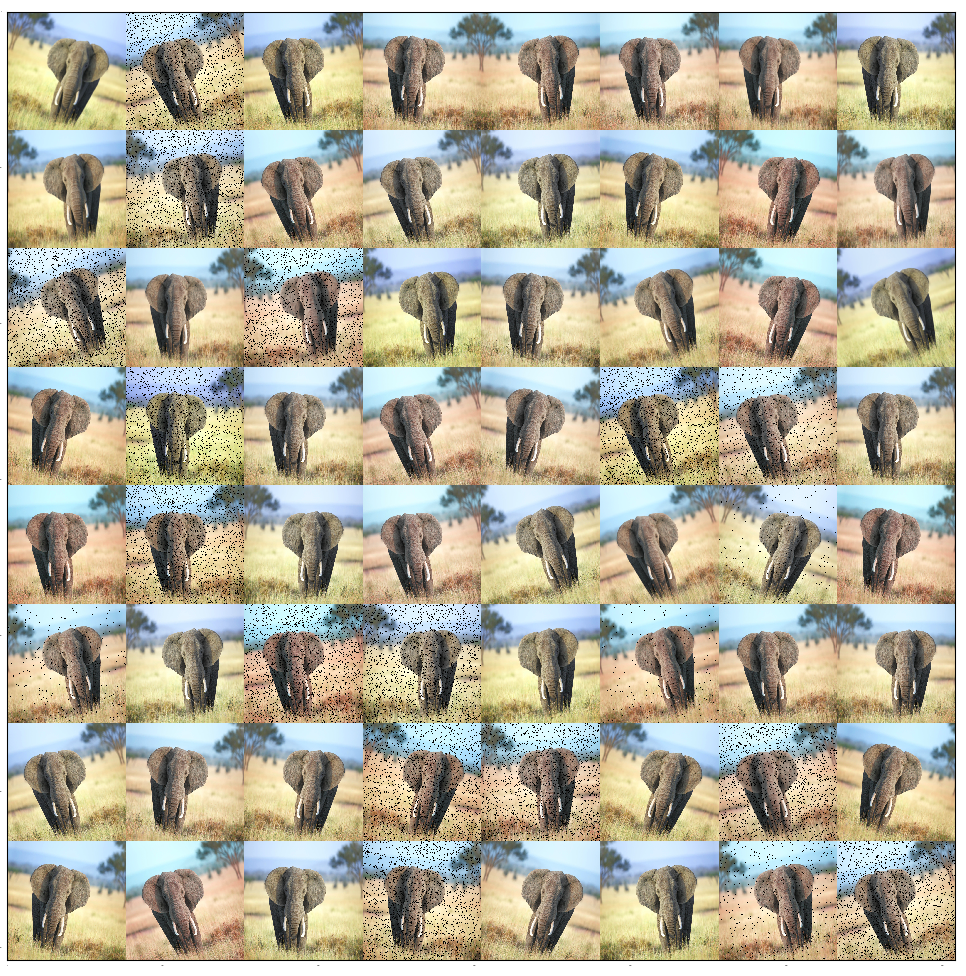
\includegraphics[width=.7\linewidth]{figures/augmentation/augmentation_high_resolution.png}
		\caption[Image Augmentaion Example]{Image Augmentation of an elephant}
		\label{fig:augmentation}
	\end{figure}
	
	Image augmentation involves transformations using tools from image processing to randomly apply noise injection, and color space transformations including contrast and saturation distortions, as well as geometric transformations, such as simple transformations of flipping the image to more complex affine transformations to create different image perspectives \cite{shorten_survey_2019}. Figure \ref{fig:augmentation} shows 64 random augmentations of an image of an elephant, achieved using \gls{imgaug} \cite{jung_imgaug:_nodate}. 
	
	New methods have been proposed where image transformations are learned to improve generalization e.g. AutoAugment \cite{cubuk_autoaugment:_2018}. 
	
	Other methods involves actually enlarging the training dataset by synthetically creating more data using a \gls{gan}. \gls{gan}s can help overcome limited data given the available training data or a 3D model, by artificially constructing new samples in different background, light setting and from alternate perspectives.
	
	Methods that do not cover enriching the available training, but alters the learning procedure are called regularization and covers; weight decay, dropout, batch normalization etc.
	
	\item[Transfer Learning] Transfer learning is the procedure of using a pre-trained model to train on a new dataset. Under the assumption, that features learned on one image dataset can be reused for another dataset \cite{yosinski_how_2014}. Transfer learning can reduce the needed time to learn general features and possibly learn better ones. Typically models have been pre-trained on the ImageNet dataset. The density of the dataset, enables model to learn general features suitable for many other domains \cite{kornblith_better_2019}. Transfer learning are especially suited for when the new data domain is of limited quantity and when the similarities between the two data domains are strong. If the similarity is less strong a model can be partially trained, the shallow layers containing general features are frozen and only the deeper layers with more specialized features are fine-tuned for the new data domain \cite{li_cs231n:_2018}.
\end{description}

\subsection{Results} \label{sec:training-results}

We trained B-\gls{resnet} using transfer learning from the ImageNet dataset. We froze the features of the network and only trained the classifiers of all the exits. Figure \ref{fig:frozen-b-resnet-miniimagenet-100} show the results from the training. The figure shows, that the features learn from a conventional model are not suitable for an early exit model. None of the intermediate classifiers are able to obtain acceptable accuracy on neither the training nor the validation set. The features for the shallower part of the network are not trained for the early classifiers. This study clearly reveals the need to train the entire model to obtain an early exit model with decent accuracy.  

\begin{figure}
	\centering
	\captionsetup[subfigure]{justification=centering, farskip=1pt,captionskip=1pt}
	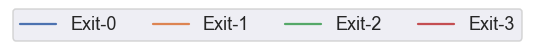
\includegraphics[width=.5\textwidth]{figures/training_plots/frozen_b-resnet_exit_legend}
	\subfloat[Train loss\label{fig:frozen-b-resnet-train-loss}]{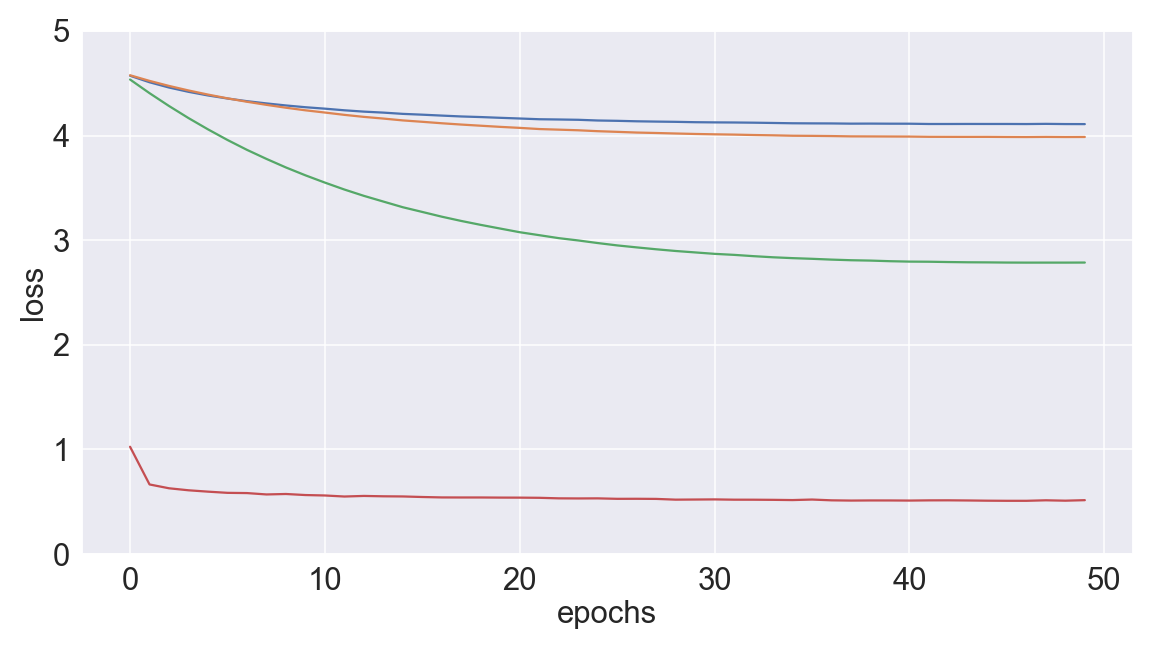
\includegraphics[width=.49\textwidth]{figures/training_plots/frozen_b-resnet_train-loss}}
	\subfloat[Test loss \label{fig:frozen-b-resnet-test-loss}]{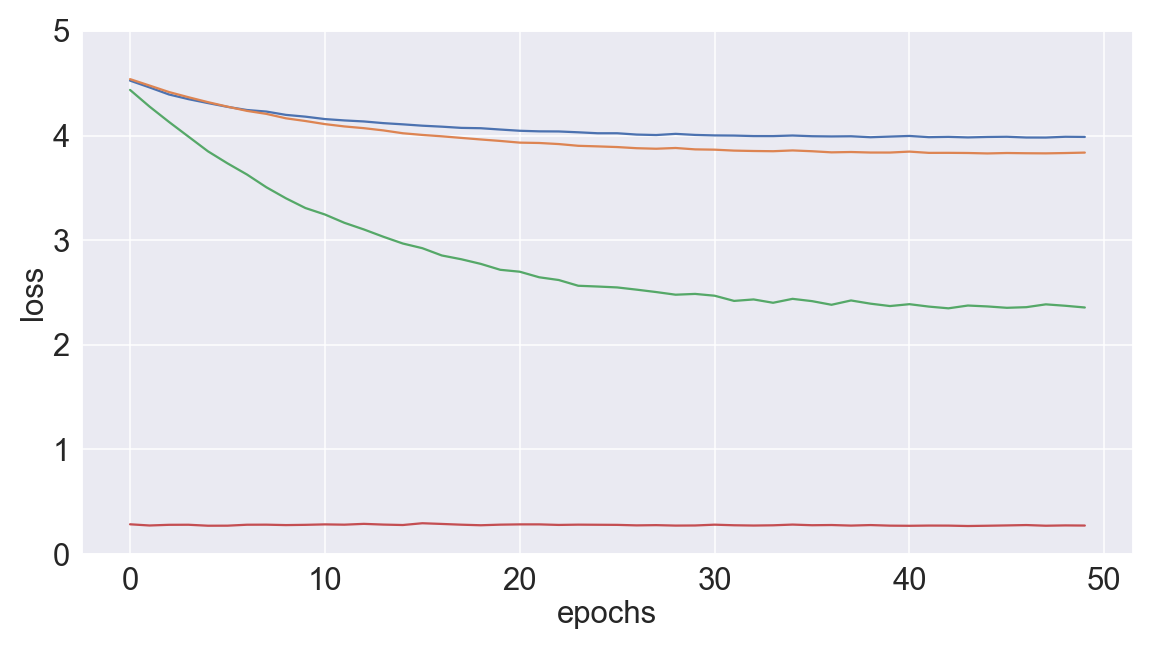
\includegraphics[width=.49\textwidth]{figures/training_plots/frozen_b-resnet_test-loss}}
	\hfill
	\subfloat[Train accuracy\label{fig:frozen-b-resnet-train-acc}]{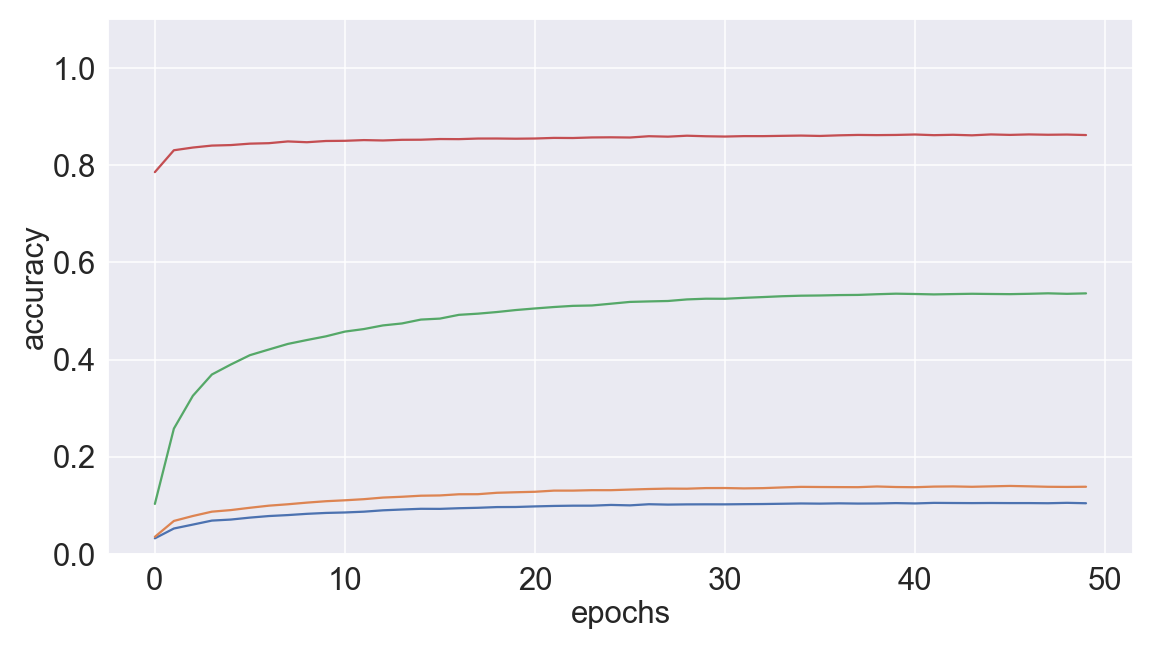
\includegraphics[width=.49\textwidth]{figures/training_plots/frozen_b-resnet_train-accuracy}}
	\subfloat[Test accuracy\label{fig:frozen-b-resnet-test-acc}]{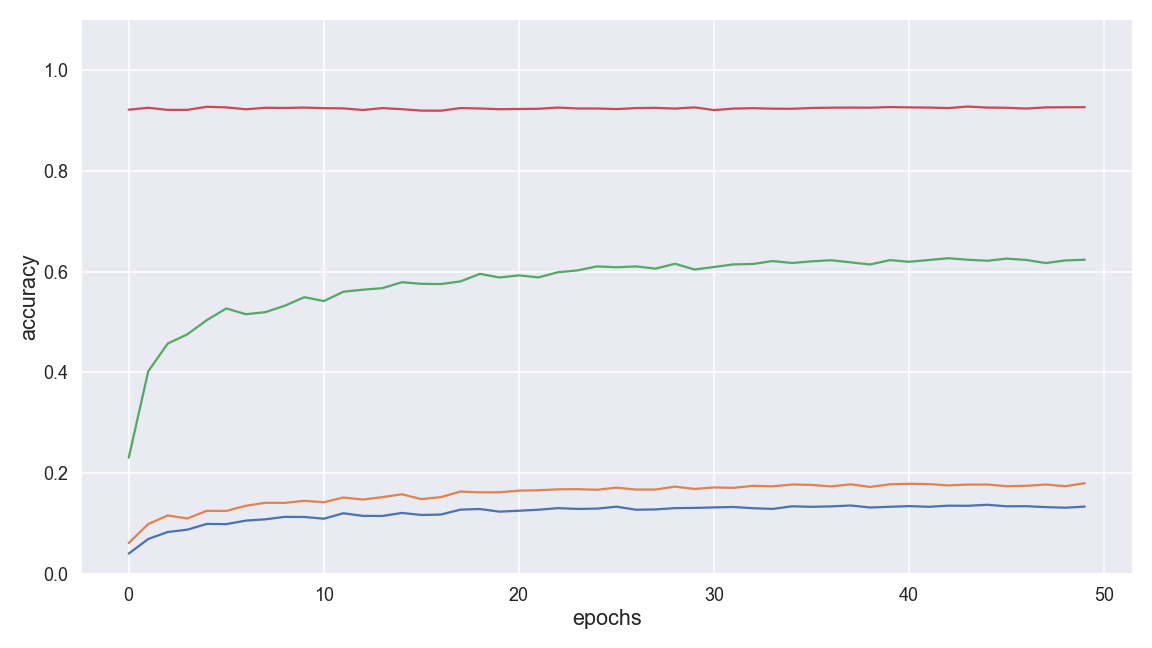
\includegraphics[width=.49\textwidth]{figures/training_plots/frozen_b-resnet_test-accuracy}}
	\caption[Frozen Bresnet Training summary]{Frozen B-resnet Training summary: shows the progression of model attributes over times of epochs, \protect\subref{fig:frozen-b-resnet-train-loss} train loss, \protect\subref{fig:frozen-b-resnet-test-loss} test loss, \protect\subref{fig:frozen-b-resnet-train-acc} train accuracy, \protect\subref{fig:frozen-b-resnet-test-acc}, test accuracy.}
	\label{fig:frozen-b-resnet-miniimagenet-100}
\end{figure}

As found in \cite{teerapittayanon_branchynet:_2016}, we unfreeze the model, to allow the features of the model to better suit the intermediate classifiers. Figure \ref{fig:b-resnet-miniimagenet-100} show the training results. 

\begin{figure}
	\centering
	\captionsetup[subfigure]{justification=centering, farskip=1pt,captionskip=1pt}
	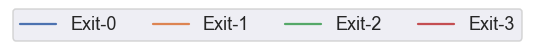
\includegraphics[width=.5\textwidth]{figures/training_plots/b-resnet_exit_legend}
	\subfloat[Train loss\label{fig:b-resnet-train-loss}]{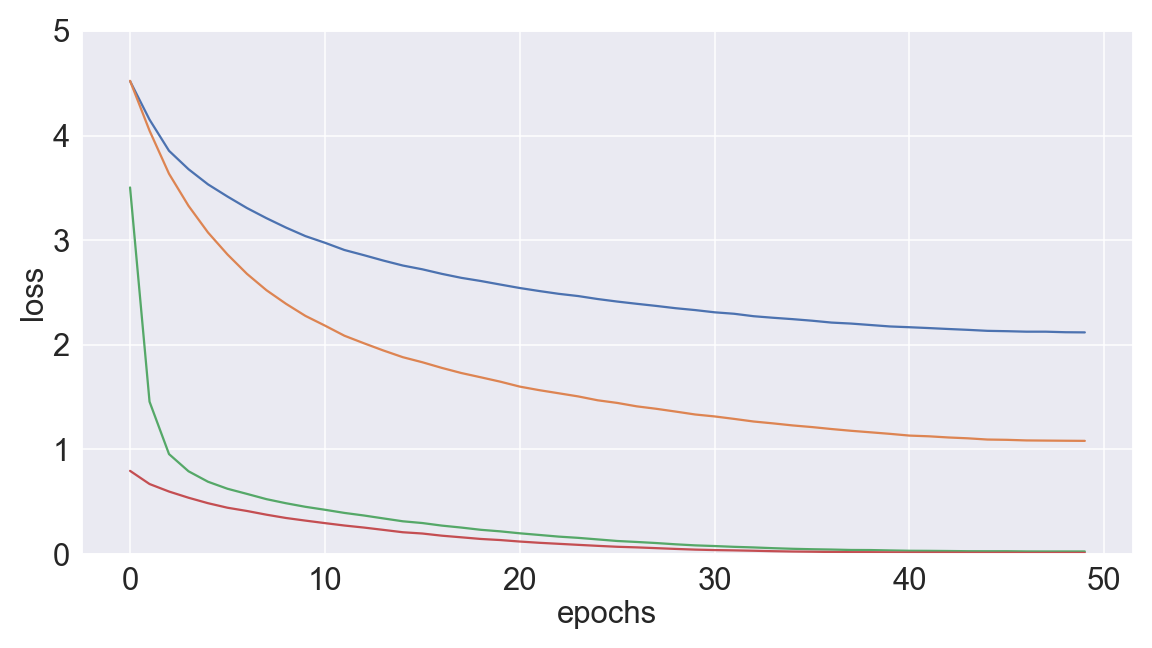
\includegraphics[width=.49\textwidth]{figures/training_plots/b-resnet_train-loss}}
	\subfloat[Test loss \label{fig:b-resnet-test-loss}]{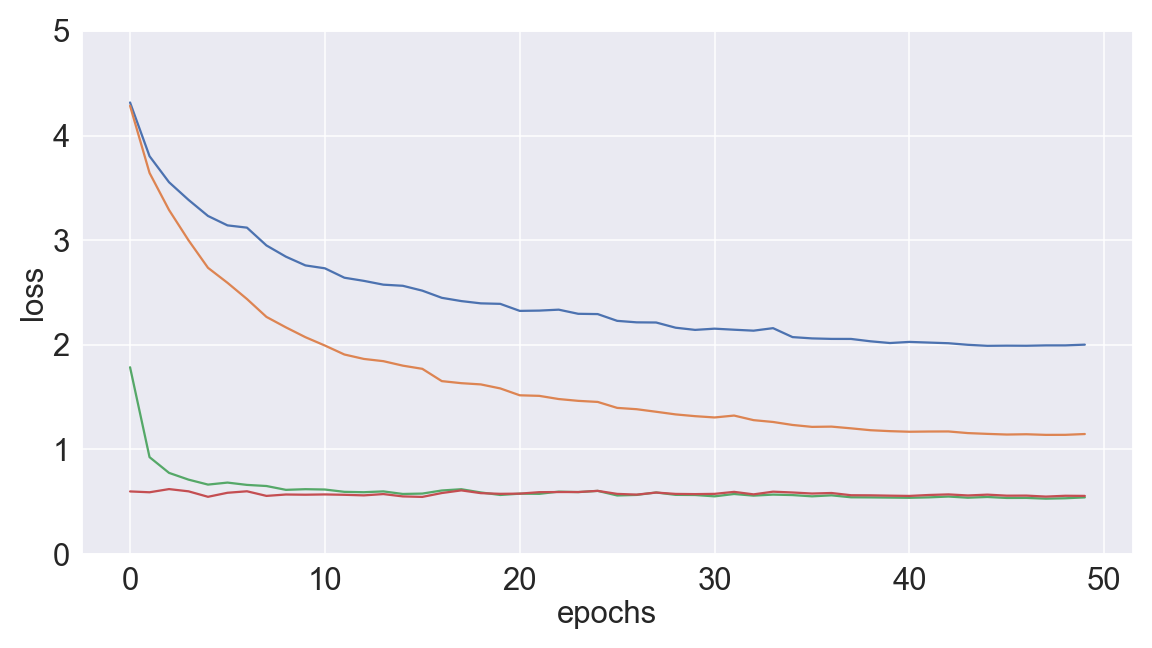
\includegraphics[width=.49\textwidth]{figures/training_plots/b-resnet_test-loss}}
	\hfill
	\subfloat[Train accuracy\label{fig:b-resnet-train-acc}]{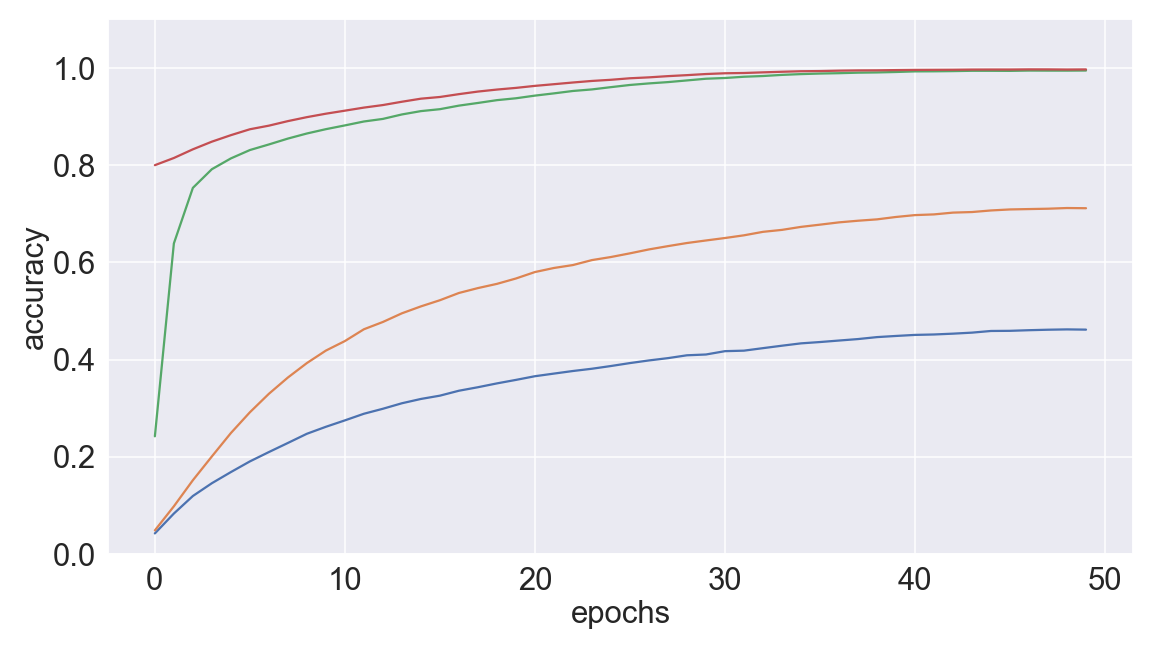
\includegraphics[width=.49\textwidth]{figures/training_plots/b-resnet_train-accuracy}}
	\subfloat[Test accuracy\label{fig:b-resnet-test-acc}]{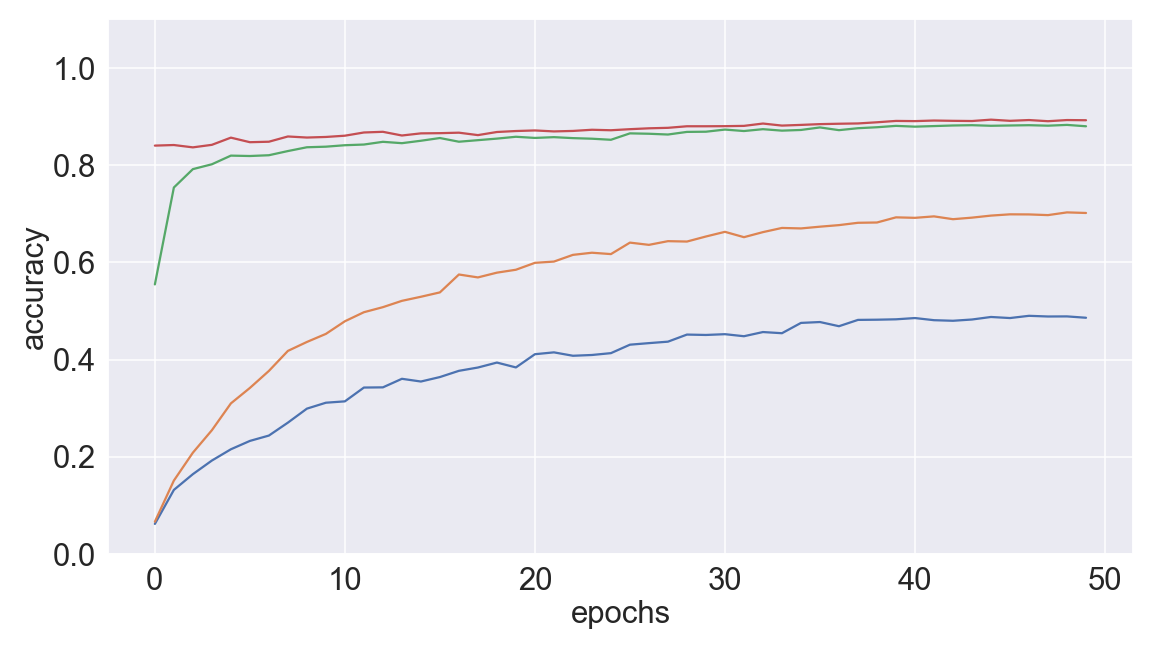
\includegraphics[width=.49\textwidth]{figures/training_plots/b-resnet_test-accuracy}}
	\caption[B-ResNet Training summary]{B-ResNet Training summary: shows the progression of model attributes over times of epochs, \protect\subref{fig:b-resnet-train-loss} train loss, \protect\subref{fig:b-resnet-test-loss} test loss, \protect\subref{fig:b-resnet-train-acc} train accuracy, \protect\subref{fig:b-resnet-test-acc}, test accuracy.}
	\label{fig:b-resnet-miniimagenet-100}
\end{figure}

Table \ref{tbl:frozen-vs-unfrozen}  shows the improvement of the higest validation score obtained in the training process. Comparing the two show, that we are now able to improve the accuracy at early exits, thus the features located in the shallower part of the model now provides information that enables the classifiers to discriminate the classes. 
\begin{longtabu}{>{\bfseries}X[2]|X|X|X|X}
	\caption[Comparison of Transfer Learning Approaches]{Comparison of transfer learning approaches frozen model vs. fine-tuning} \label{tbl:frozen-vs-unfrozen} \\
	\toprule
	\rowfont{\bfseries}
	Model & Exit-0 & Exit-1 & Exit-2 & Exit-1 \tabularnewline
	\bottomrule
	\endfirsthead
	\multicolumn{3}{@{}l}{\textbf{\textcolor{black}{Table \ref{tbl:frozen-vs-unfrozen}:}} continued}\\
	\toprule
	\rowfont{\bfseries}
	Model & Exit-0 & Exit-1 & Exit-2 & Exit-1 \tabularnewline
	\bottomrule
	\endhead % all the lines above this will be repeated on every page
	\bottomrule
	\multicolumn{3}{@{}l}{continued \ldots}\\
	\endfoot
	\hline
	\endlastfoot
	Frozen B-\gls{resnet}	& 0.14	& 0.18	& 0.63 & 0.93 \tabularnewline
	\hline
	Unfrozen B-\gls{resnet}	& 0.49 	& 0.70 & 0.88 & 0.89 \tabularnewline
	\hline
	Improvement & 350 \% & 389 \% & 140 \% &  96 \% \tabularnewline							
	\bottomrule
\end{longtabu}
Although the final classifier have become less accurate by 4 \%, the early classifiers have been improved by 140 to almost 390 \%. The reduction in accuracy may be caused by the rather large resolution block before exit-2, the features of this block may be optimized to much for exit-2 and collapses the information, that the last resolution block learns for the conventional model. The two last exits of \gls{resnet} are almost equally accurate. Thus, not much gain in accuracy is obtained by running \gls{resnet} model all the way to the end. \gls{densenet} on the other hand always have an accuracy gain by continuing the inference process.     

\begin{figure}
	\centering
	\captionsetup[subfigure]{justification=centering, farskip=1pt,captionskip=1pt}
	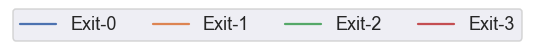
\includegraphics[width=.5\textwidth]{figures/training_plots/b-densenet_exit_legend}
	\subfloat[Train loss\label{fig:b-densenet-train-loss}]{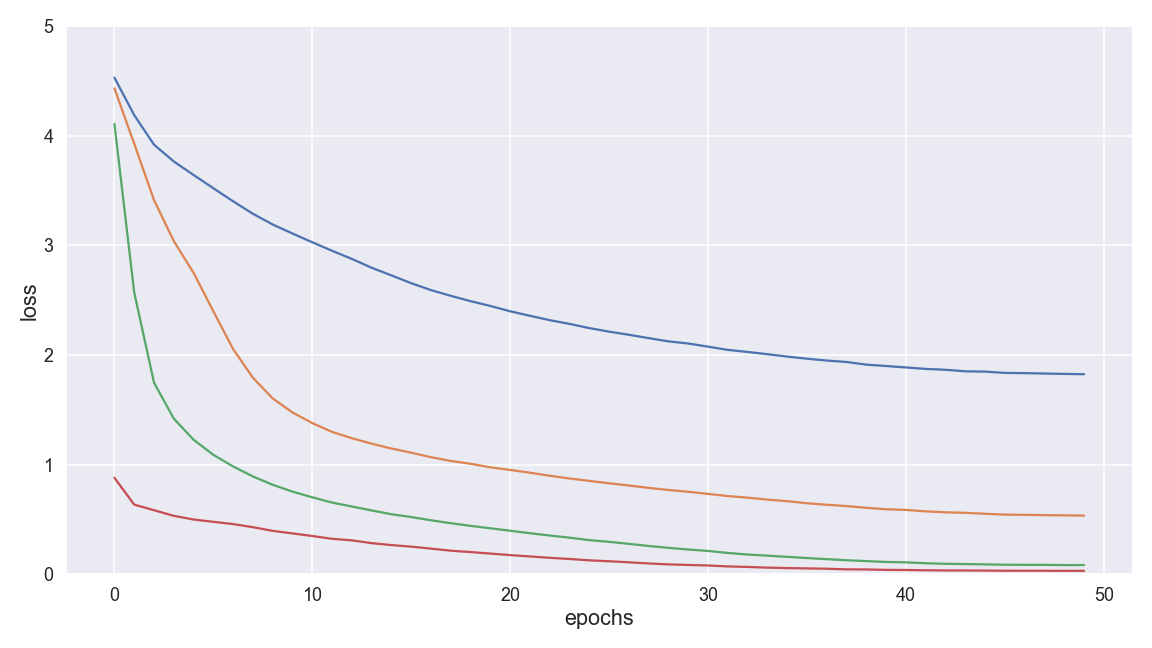
\includegraphics[width=.49\textwidth]{figures/training_plots/b-densenet_train-loss}}
	\subfloat[Test loss \label{fig:b-densenet-test-loss}]{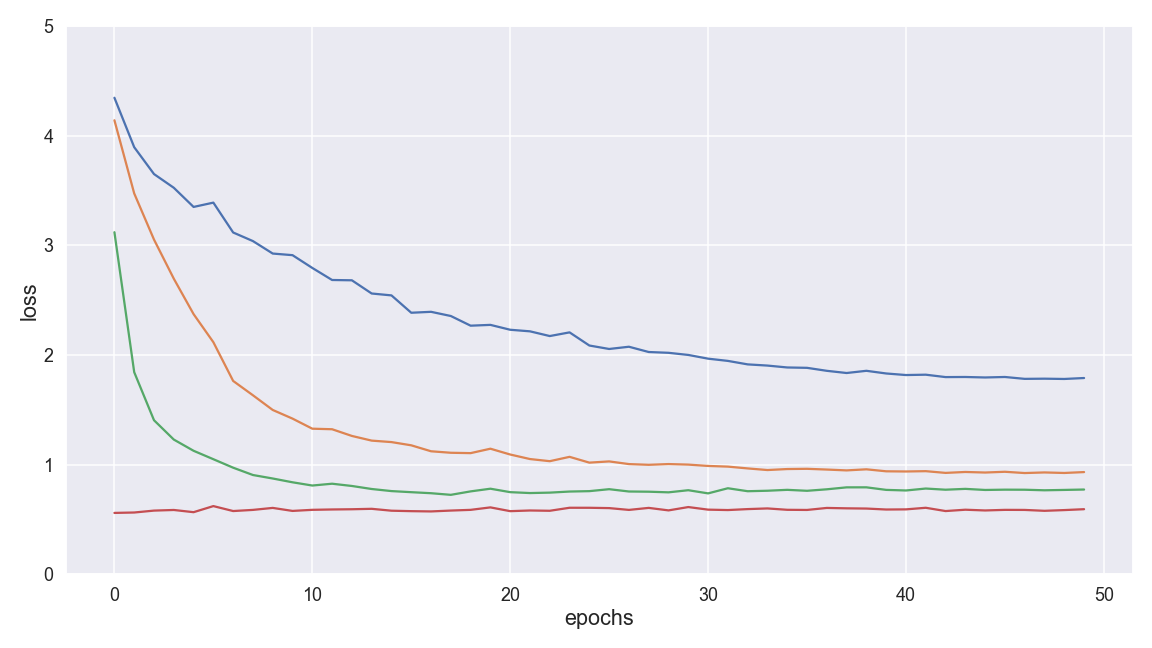
\includegraphics[width=.49\textwidth]{figures/training_plots/b-densenet_test-loss}}
	\hfill
	\subfloat[Train accuracy\label{fig:b-densenet-train-acc}]{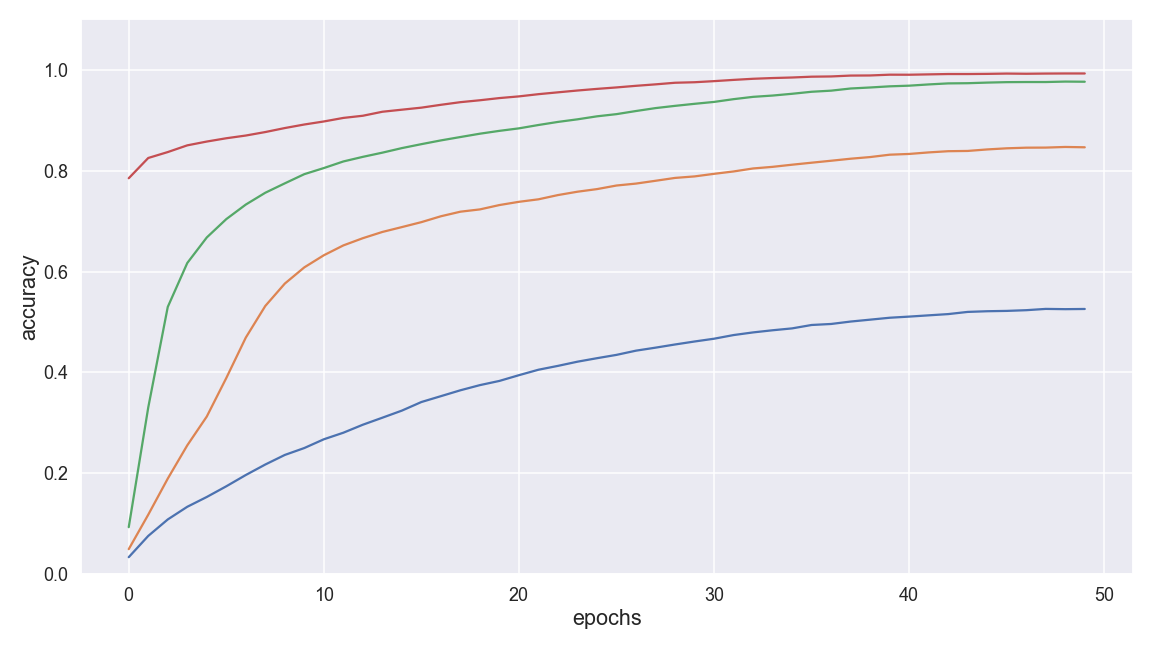
\includegraphics[width=.49\textwidth]{figures/training_plots/b-densenet_train-accuracy}}
	\subfloat[Test accuracy\label{fig:b-densenet-test-acc}]{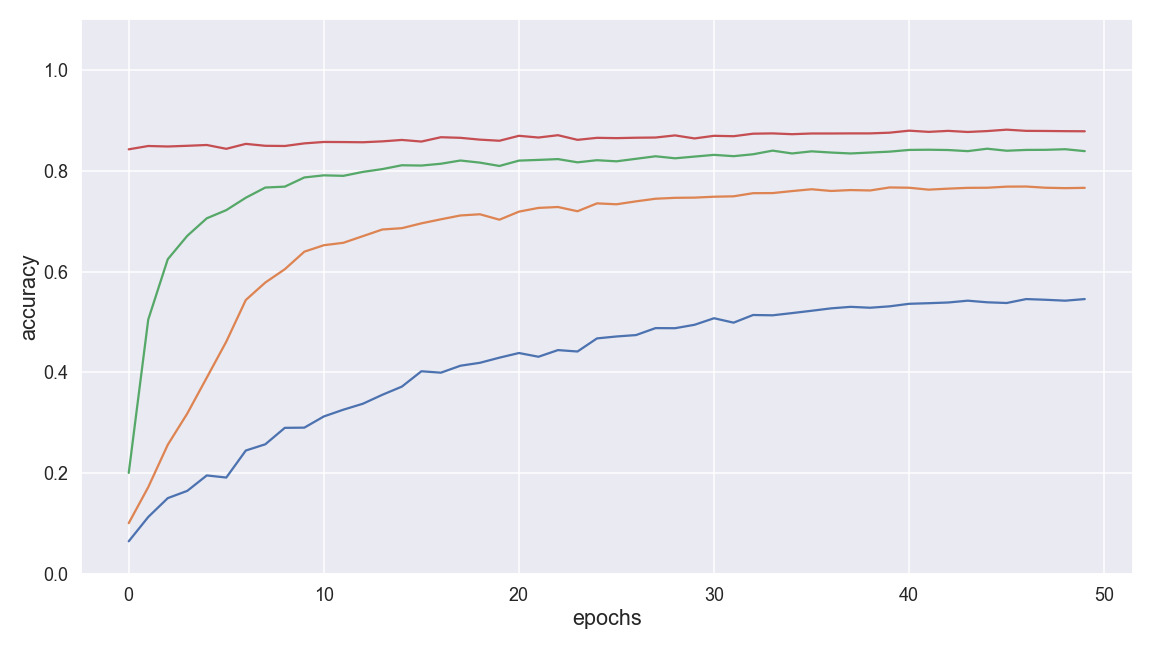
\includegraphics[width=.49\textwidth]{figures/training_plots/b-densenet_test-accuracy}}
	\caption[B-densenet Training summary]{B-densenet Training summary: shows the progression of model attributes over times of epochs, \protect\subref{fig:b-densenet-train-loss} train loss, \protect\subref{fig:b-densenet-test-loss} test loss, \protect\subref{fig:b-densenet-train-acc} train accuracy, \protect\subref{fig:b-densenet-test-acc}, test accuracy.}
	\label{fig:b-densenet-miniimagenet-100}
\end{figure}

Figure \ref{fig:b-densenet-miniimagenet-100} show the training result of B-\gls{densenet}. The early exits of the model show further improvement compared to B-\gls{resnet}, however again at the cost of less accurate end exit. The figure shows the importance of the densely connected layers for an early exit model \cite{huang_multi-scale_2017}. The early exits of B-\gls{densenet} have a higher accuracy compared to B-\gls{resnet}, but the last two exits of  B-\gls{resnet} obtain higher accuracy, see table \ref{tbl:training-compariosn}. \gls{msdnet}, the early exiting version of \gls{densenet}, shows further improvement to early exits accuracy.

\begin{figure}
	\centering
	\captionsetup[subfigure]{justification=centering, farskip=1pt,captionskip=1pt}
	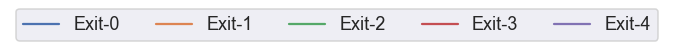
\includegraphics[width=.5\textwidth]{figures/training_plots/msdnet_exit_legend}
	\subfloat[Train loss\label{fig:msdnet-train-loss}]{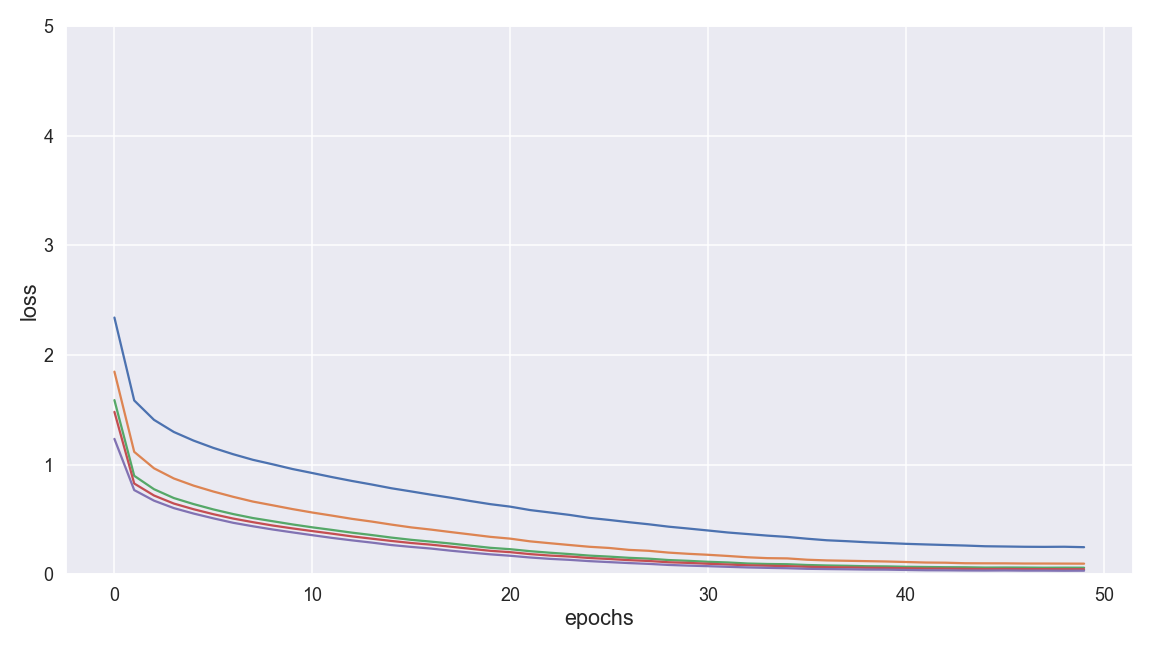
\includegraphics[width=.49\textwidth]{figures/training_plots/msdnet_train-loss}}
	\subfloat[Test loss \label{fig:msdnet-test-loss}]{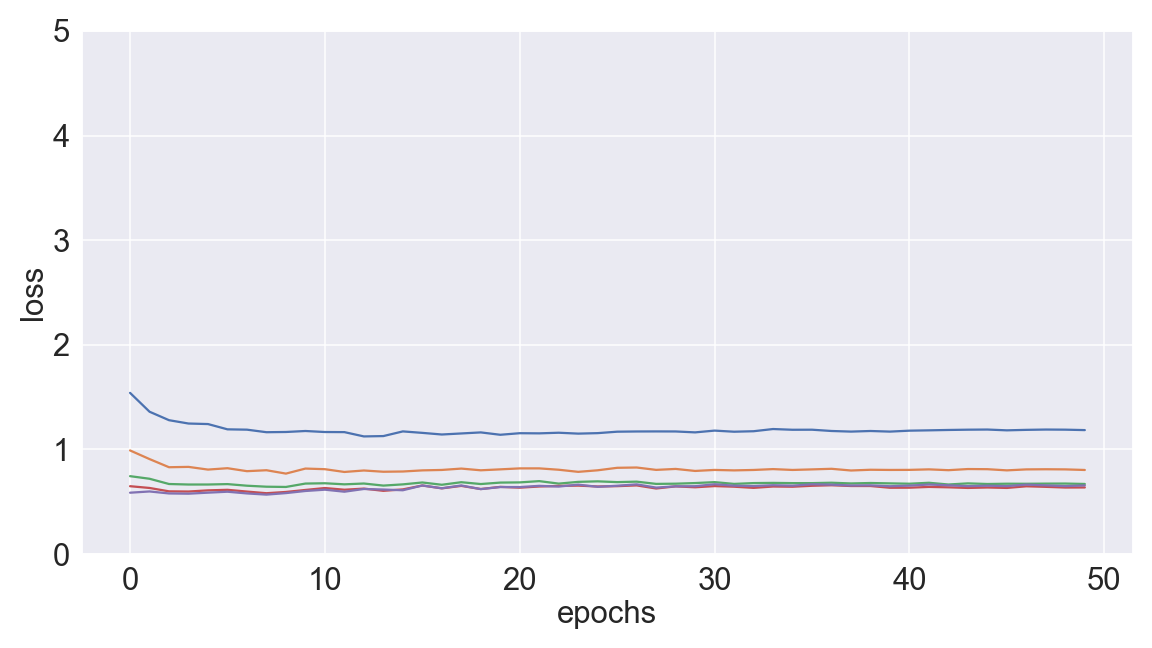
\includegraphics[width=.49\textwidth]{figures/training_plots/msdnet_test-loss}}
	\hfill
	\subfloat[Train accuracy\label{fig:msdnet-train-acc}]{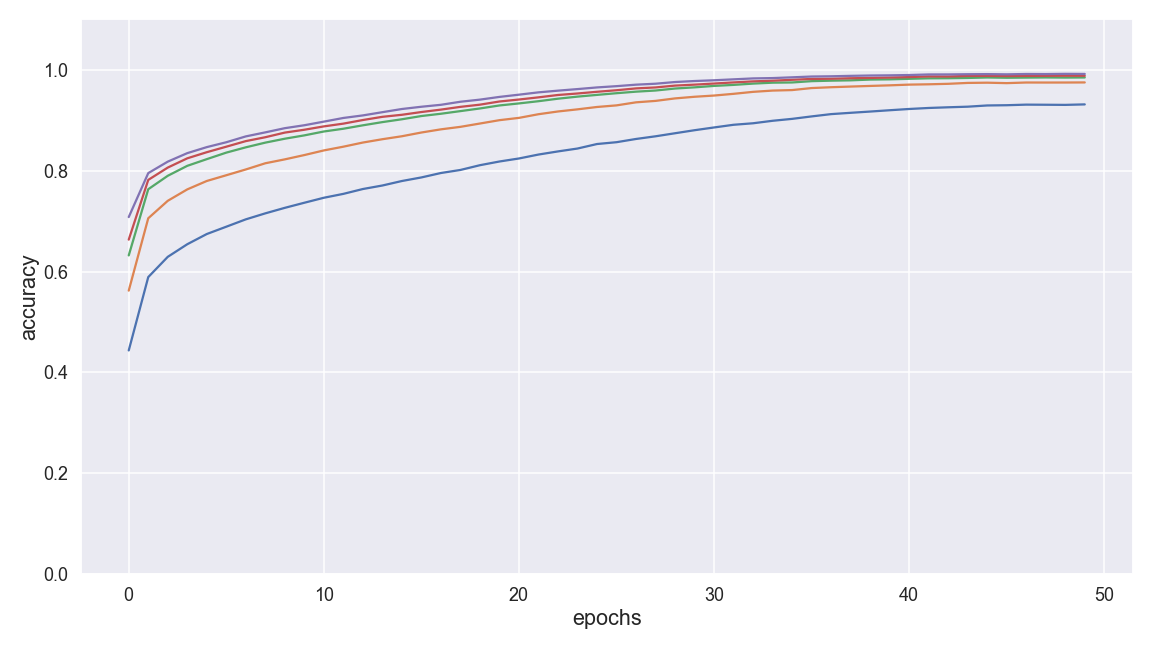
\includegraphics[width=.49\textwidth]{figures/training_plots/msdnet_train-accuracy}}
	\subfloat[Test accuracy\label{fig:msdnet-test-acc}]{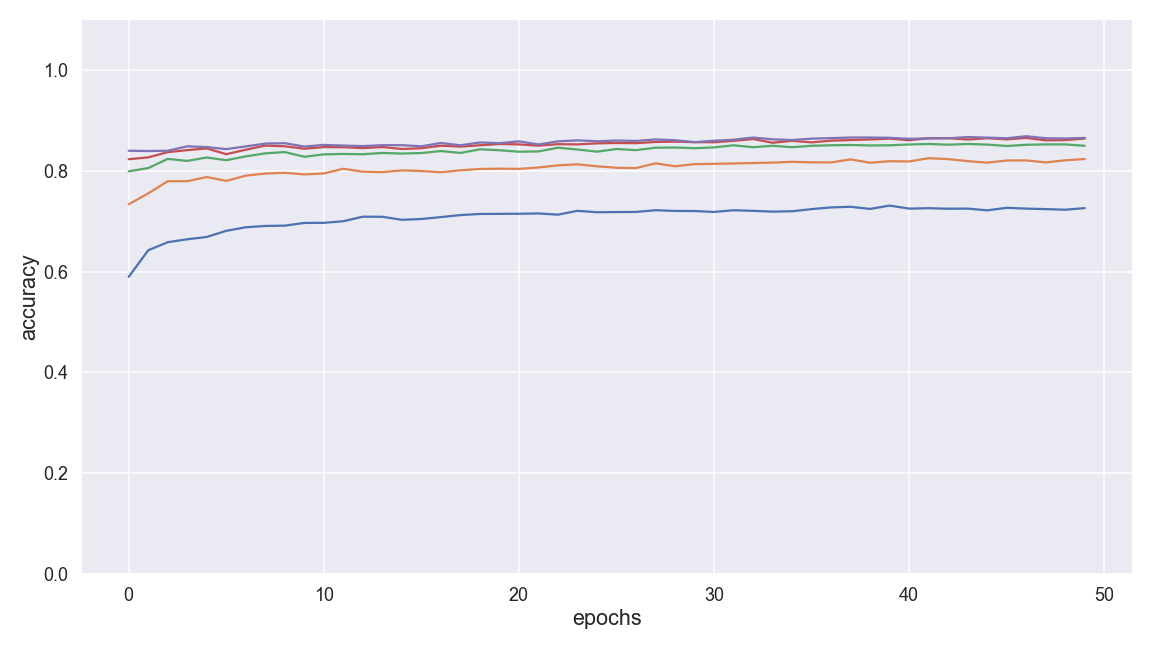
\includegraphics[width=.49\textwidth]{figures/training_plots/msdnet_test-accuracy}}
	\caption[MSDNet Training summary]{MSDNet Training summary: shows the progression of model attributes over times of epochs, \protect\subref{fig:msdnet-train-loss} train loss, \protect\subref{fig:msdnet-test-loss} test loss, \protect\subref{fig:msdnet-train-acc} train accuracy, \protect\subref{fig:msdnet-test-acc}, test accuracy.}
	\label{fig:msdnet-miniimagenet-100}
\end{figure}

Figure \ref{fig:msdnet-miniimagenet-100} show the results of training the \gls{msdnet}. The model specifically designed for early exiting shows indeed improvement for classifiers at early exit, but once again at a small cost in end accuracy compared to the other two models. Table \ref{tbl:training-compariosn} compares the best obtained validation accuracy in the training processes of the three models.


\begin{longtabu}{>{\bfseries}X[2]|X|X|X|X|X}
	\caption[Early Exiting Validation Accuracy from Training]{Early Exiting Validation Accuracy from Training} \label{tbl:training-compariosn} \\
	\toprule
	\rowfont{\bfseries}
	Model & Exit-0 & Exit-1 & Exit-2 & Exit-3 & Exit-4 \tabularnewline
	\bottomrule
	\endfirsthead
	\multicolumn{3}{@{}l}{\textbf{\textcolor{black}{Table \ref{tbl:frozen-vs-unfrozen}:}} continued}\\
	\toprule
	\rowfont{\bfseries}
	Model & Exit-0 & Exit-1 & Exit-2 & Exit-3 & Exit-4 \tabularnewline
	\bottomrule
	\endhead % all the lines above this will be repeated on every page
	\bottomrule
	\multicolumn{3}{@{}l}{continued \ldots}\\
	\endfoot
	\hline
	\endlastfoot
	B-\gls{resnet} & 0.49 	& 0.70 & 0.88 & 0.89 & N/A \tabularnewline
	\hline
	B-\gls{densenet}	& 0.55 	& 0.77 & 0.84 & 0.88 & N/A \tabularnewline
	\hline
	\gls{msdnet} & 0.73 & 0.82 & 0.85 &  0.87 & 0.87 \tabularnewline							
	\bottomrule
\end{longtabu}

In the next section we evaluate the trained models on the \gls{min100} validation set.

\subsection{Validation Analysis}

In this section we evaluate the accuracy of the early exit models. All validation samples are inferred to all exits of the three models. Figure \ref{fig:exit-accuracy} show top-1 and top-5 accuracy of all exits of the three models. Fortunately we get similar results to the training.  

\begin{figure}
	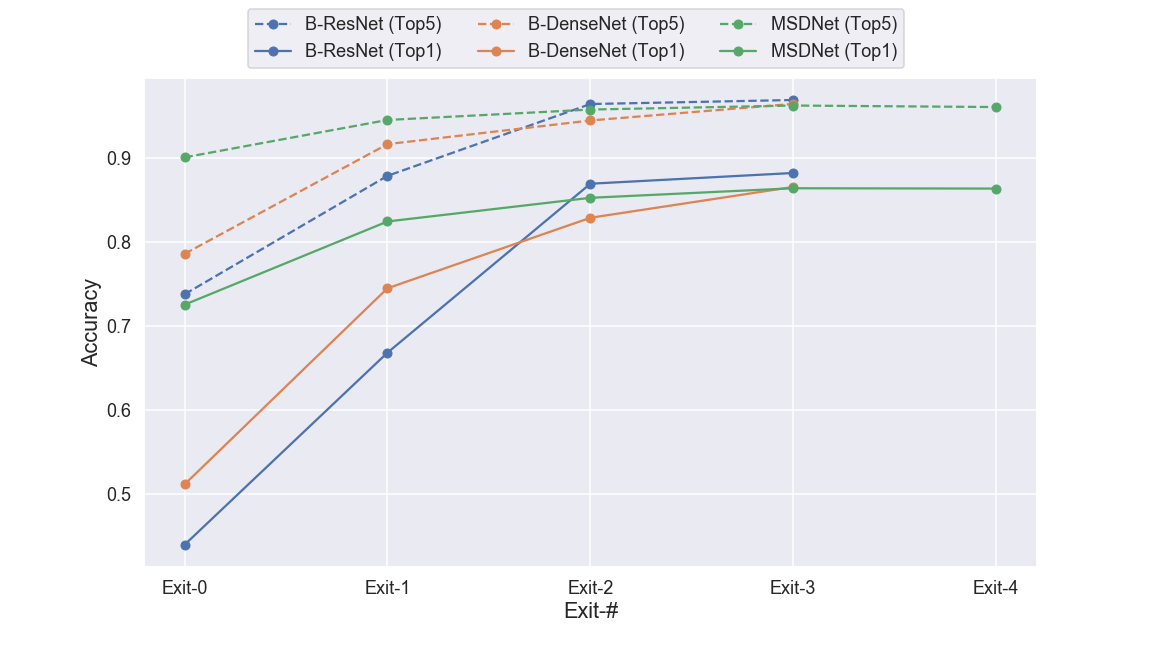
\includegraphics[width=\linewidth]{figures/inference_plots/accuracy-comparison}
	\caption[Accuracy of Early Exit Models]{Accuracy of Early Exit Models, B-\gls{resnet}, B-\gls{densenet} and \gls{msdnet}}
	\label{fig:exit-accuracy}
\end{figure}

As expected the models become more accurate as we go deeper in the network, as the increasingly complex features deep within the network have more discriminative characteristics. As stated in \cite{huang_multi-scale_2017} the densely connected features are important factors for obtaining intermediate classifiers with decent accuracy. The B-\gls{densenet} and \gls{msdnet} have as expected more accurate early classifiers, however the end-exit of B-\gls{resnet} achieves superior top-1 accuracy compared to the other models.

Still close to 50 \% of the samples can be accurately classified by any of the models at the very first exit, which justifies the assumption for \gls{branchynet} and promisingly we should be able to save time. 

\section{Early Exit Analysis} \label{sec:early-exit-analysis}

In this section we investigates the early exiting capabilities of the models. Table \ref{tbl:early-exit} compares the models' accuracy, number of layers, number of parameters and the number of \gls{flop}s required by model inference.

\begin{longtabu}{>{\bfseries}X|X[r]|X[r]|X[r]|X[r]}
	\caption[Early exit models' last exit accuracy]{Early exit models' last exit accuracy. Model Parametric Comparison using \texttt{thop} \cite{zhu_thop_nodate}. The test is conducted by inference a random 4d tensor of size $ (\mathrm{batch,channels,width,height})=(1,3,224,224) $ to all models.}\label{tbl:early-exit} \\
	\toprule
	\rowfont{\bfseries}
	Model & Accuracy  & Layers & Parameters (M) & G\gls{flop}s \tabularnewline
	\hline
	\endfirsthead
	\multicolumn{3}{@{}l}{\textbf{\textcolor{black}{Table \ref{tbl:early-exit}:}} continued}\\
	\toprule
	\rowfont{\bfseries}
	Model & Accuracy & Layers & Parameters (M) & G\gls{flop}s \tabularnewline
	\hline
	\endhead % all the lines above this will be repeated on every page
	\hline
	\multicolumn{3}{@{}l}{continued \ldots}\\
	\endfoot
	\hline
	\endlastfoot
	ResNet  & 0.929 & $ 101 $ & $ 42.705 $ & $ 7.864 $ \tabularnewline
	\hline
	DenseNet & 0.912 & $ 121 $ & $ 7.056 $ & $ 2.897 $ \tabularnewline
	\hline
	B-ResNet & & $ 107 $ & $ 42.885 $ & $ 7.866 $ \tabularnewline 
	\hspace{3mm} Exit-0 & 0.489  & & & \tabularnewline
	\hspace{3mm} Exit-1 & 0.703  & & &\tabularnewline
	\hspace{3mm} Exit-2 & 0.883  & & &\tabularnewline
	\hspace{3mm} Exit-3 & 0.893  & & &\tabularnewline
	\hline
	B-DenseNet &  & $ 127 $ & $ 7.236 $ & $ 2.898 $\tabularnewline
	\hspace{3mm} Exit-0 & 0.545 & & & \tabularnewline
	\hspace{3mm} Exit-1 & 0.769 & & &\tabularnewline
	\hspace{3mm} Exit-2 & 0.841 & & &\tabularnewline
	\hspace{3mm} Exit-3 & 0.879 & & &\tabularnewline
	\hline
	MSDNet & & $ 24 $ & $ 23.958 $ & $ 1.374 $ \tabularnewline
	\hspace{3mm} Exit-0 & 0.755 & & &\tabularnewline
	\hspace{3mm} Exit-1 & 0.829 & & &\tabularnewline
	\hspace{3mm} Exit-2 & 0.859 & & &\tabularnewline
	\hspace{3mm} Exit-3 & 0.864 & & &\tabularnewline
	\hspace{3mm} Exit-4 & 0.867 & & &\tabularnewline
	\bottomrule
\end{longtabu}

Interestingly the B-\gls{densenet} and \gls{msdnet} drastically reduces the mount of parameters and G\gls{flop}s compared to B-\gls{resnet}, but is still able to obtain competitive accuracy. The two conventional models \gls{resnet} and \gls{densenet} outperforms the early exiting model in terms of accuracy, however the models are inflexible, as they always require end-to-end inference. The early exit models should be able to reduce inference delay, as they need less parameters and \gls{flop}s.

In the next section we describe the experimental setup used throughout the early exiting analyses.

\subsection{Experimental Setup}

\begin{longtabu}{>{\bfseries}X[0.8]|X[0.8]|X[1.5]|X[r0.3]}
	\caption[Platform hardware comparison]{Platform hardware comparison of Window 10 Stationary PC and NVIDIA Jetson TX2 Edge Computer} \label{tbl:platforms} \\
	\toprule
	\rowfont{\bfseries}
	Platform & CPU & GPU & RAM  \tabularnewline
	\bottomrule
	\endfirsthead
	\multicolumn{3}{@{}l}{\textbf{\textcolor{black}{Table \ref{tbl:platforms}:}} continued}\\
	\toprule
	\rowfont{\bfseries}
	Platform & CPU & GPU & RAM  \tabularnewline
	\bottomrule
	\endhead % all the lines above this will be repeated on every page
	\bottomrule
	\multicolumn{3}{@{}l}{continued \ldots}\\
	\endfoot
	\hline
	\endlastfoot
	Windows PC	& Intel i5-6600K.	& NVIDIA GeForce GTX 1080, 2560 CUDA cores	& 16GB \tabularnewline
	\hline
	Jetson TX2	& ARM Cortex-A57 	& NVIDIA Pascal GPU, 256 CUDA cores 		& 8GB \tabularnewline
	\hline
	NUC		  	& Intel i7-7567U	& None										& 16GB \tabularnewline									
	\bottomrule
\end{longtabu}

In the next section we conduct a practical experiment by timing all exit prediction of the three early exit models and the two conventional model for benchmarking. 

\subsection{Inference Latency Analysis}

We setup a test, where we inference the entire \gls{min100} validation set the in all 5 models on three different platforms. Table \ref{tbl:inference-stats} show statistical values mean, standard deviation, minimum and maximum for the model inference time on the different platforms. From the table one can see, that the early exiting framework adds additional delay when using the last exit of the compared to the models conventional pendant.  
\begin{longtabu}{>{\bfseries}X[2.6]|[1pt]X[r]|X[0.8r]|X[r]|X[r]|[1pt]X[r]|X[0.8r]|X[r]|X[r]|[1pt]X[r]|X[0.8r]|X[r]|X[r]}
	\caption[Inference time statistics]{Inference time statistics (mean, standard deviation, minimum, maximum) of the five models on the three platforms }\label{tbl:inference-stats} \\
	\toprule
	\rowfont{\bfseries}
	& \multicolumn4{c|[1pt]}{GPU Workstation} &  \multicolumn4{c|[1pt]}{Jetson TX2} & \multicolumn4{c}{Intel NUC} \tabularnewline
	\tabucline{2-13}
	\rowfont{\bfseries} Model & Mean & Std.  & Min & Max & Mean & Std. & Min & Max & Mean & Std.  & Min & Max  \tabularnewline
	\hline
	\endfirsthead
	\multicolumn{3}{@{}l}{\textbf{\textcolor{black}{Table \ref{tbl:inference-stats}:}} continued}\\
	\toprule
	\rowfont{\bfseries}
	& \multicolumn4{c|[1pt]}{GPU Workstation} &  \multicolumn4{c|[1pt]}{Jetson TX2} & \multicolumn4{c}{Intel NUC} \tabularnewline
	\tabucline{2-13}
	\rowfont{\bfseries} Model & Mean & Std.  & Min & Max & Mean & Std.  & Min & Max & Mean & Std.  & Min & Max  \tabularnewline
	\hline
	\endhead % all the lines above this will be repeated on every page
	\hline
	\multicolumn{3}{@{}l}{continued \ldots}\\
	\endfoot
	\hline
	\endlastfoot
	ResNet  	& 44.55 & 2.69 & 40.09 &  85.83 & 64.19 & 1.95 & 61.28 & 110.17 & 215.76 & 21.98 & 132.98 & 275.55 \tabularnewline
	\hline
	DenseNet 	& 59.22 & 3.42 & 54.39 & 114.25 & 70.48 & 3.04 & 59.56 & 132.45 &  72.30 &  2.61 &  69.02 & 107.63 \tabularnewline
	\hline
	B-ResNet & & & &&&&&&&& &  \tabularnewline 
	\hspace{3mm} Exit-0 & 12.80 & 1.02 & 11.20 & 42.98 &  8.61 & 0.31 &  8.39 &  15.54 &  38.25 &  1.85 &  29.26 &  74.94 \tabularnewline
	\hspace{3mm} Exit-1 & 18.61 & 1.45 & 16.23 & 68.41 & 19.30 & 1.08 & 16.42 &  38.41 &  66.69 &  3.15 &  50.41 & 110.80 \tabularnewline
	\hspace{3mm} Exit-2 & 45.31 & 3.15 & 40.83 & 90.61 & 56.77 & 2.73 & 52.34 & 102.58 & 196.43 &  8.81 & 150.11 & 254.86 \tabularnewline
	\hspace{3mm} Exit-3 & 49.45 & 3.38 & 45.01 & 99.01 & 67.04 & 2.86 & 62.47 & 116.74 & 223.32 & 10.35 & 170.95 & 289.67 \tabularnewline
	\hline
	B-DenseNet &  & & &&&&&&&& & \tabularnewline
	\hspace{3mm} Exit-0 & 18.05 & 1.22 & 16.02 & 68.16 & 11.16 & 0.49 &	10.53 &   18.28 &  42.16 & 2.02 & 27.64 &  67.76 \tabularnewline
	\hspace{3mm} Exit-1 & 30.18 & 2.29 & 26.57 & 77.42 & 30.51 & 2.05 & 23.95 &   50.56 &  70.44 & 3.30 & 45.01 & 128.94 \tabularnewline
	\hspace{3mm} Exit-2 & 51.82 & 3.50 & 47.11 & 95.96 & 55.74 & 3.25 & 48.42 &   91.33 &  96.85 & 4.41 & 61.95 & 187.57 \tabularnewline
	\hspace{3mm} Exit-3 & 66.32 & 3.89 & 60.91 & 115.25 & 72.90 & 3.92 & 65.13 & 124.61 & 107.92 & 4.91 & 69.49 & 219.40 \tabularnewline
	\hline
	MSDNet & & &&&&&&&&&& \tabularnewline
	\hspace{3mm} Exit-0 & 38.40 & 4.53 & 34.89 &  84.85 &  40.37 & 2.77 & 29.36 & 209.89 & 19.99 & 1.27 & 16.99 &  35.12 \tabularnewline
	\hspace{3mm} Exit-1 & 59.60 & 6.00 & 55.24 & 106.53 &  65.18 & 4.29 & 53.34 & 267.19 & 32.82 & 2.38 & 29.03 & 103.19 \tabularnewline
	\hspace{3mm} Exit-2 & 75.70 & 6.99 & 70.58 & 116.71 &  83.81 & 5.43 & 71.39 & 312.55 & 42.89 & 3.03 & 38.72 & 130.52 \tabularnewline
	\hspace{3mm} Exit-3 & 86.07 & 6.79 & 81.22 & 123.35 &  96.53 & 6.26 & 83.68 & 345.67 & 50.10 & 3.43 & 45.66 & 145.75 \tabularnewline
	\hspace{3mm} Exit-4 & 91.63 & 7.71 & 86.04 & 142.07 & 103.29 & 6.65 & 90.14 & 361.02 & 56.02 & 3.62 & 51.28 & 154.08 \tabularnewline
	\bottomrule
\end{longtabu}

Figure \ref{fig:inference-time-dist} shows the result as a histogram of the inference time for a classification at the corresponding exit. The inference timings are very different on the three platforms, and is very much dependent on the hardware characteristics. The GPU Workstation are enabled with the strongest \gls{gpu}, thus have the most parallelization capabilities and able to run \gls{resnet} faster, as it requires enormous amounts of multiply-adds well-suited for \gls{gpu} acceleration. \gls{densenet} and \gls{msdnet} uses concatenation which might be a more expensive operation on the \gls{gpu}. Using only a \gls{cpu}-only device the same level of parallelization cannot be achieved to accelerate model inference. The Intel NUC, shows the opposite trend, in fact the \gls{msdnet} outperform the other models on the NUC, as it requires far fewer G\gls{flop}s and are comprised of far fewer layers and parameters.

\begin{figure}
	\begin{minipage}{\textwidth}
		\centering
		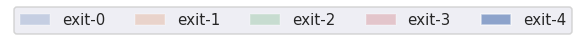
\includegraphics[width=.5\linewidth]{figures/inference_plots/time_dist_legend}
	\end{minipage}
	\begin{minipage}{0.33\textwidth}
		\captionsetup[subfigure]{farskip=0pt,captionskip=0pt, justification=centering}
		\centering
		GPU Workstation
		\subfloat[\gls{resnet} ]{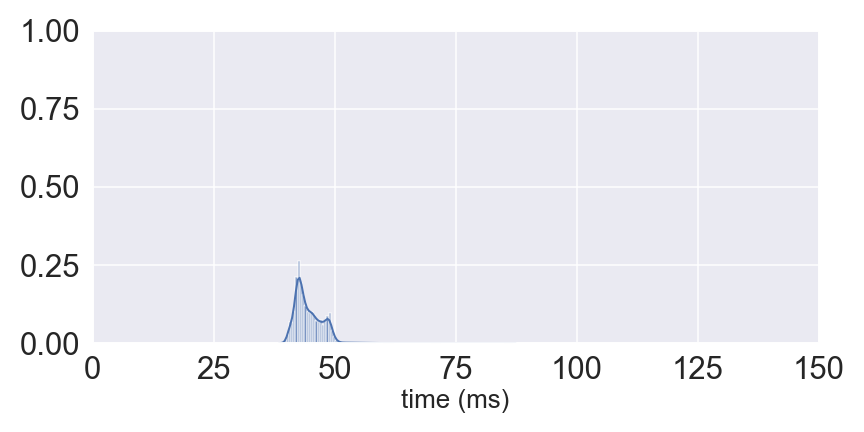
\includegraphics[width=\textwidth,height=.2\textheight,keepaspectratio]{figures/inference_plots/gpu_resnet_inference_time_distribution}}
		\hfill
		\subfloat[B-\gls{resnet}]{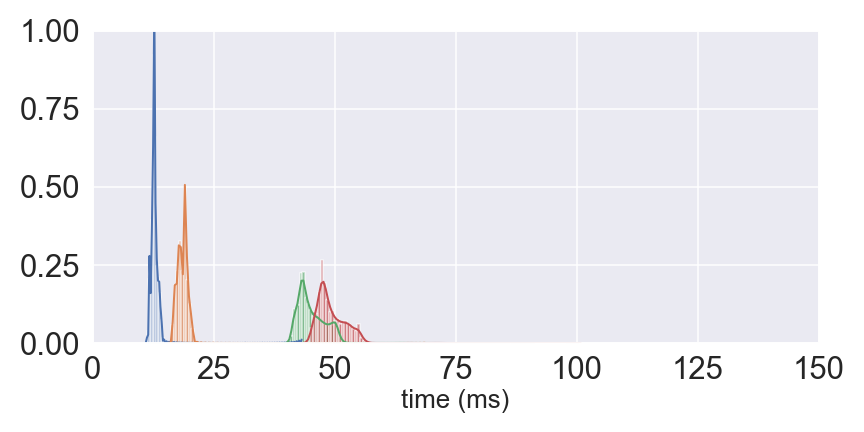
\includegraphics[width=\textwidth,height=.2\textheight,keepaspectratio]{figures/inference_plots/gpu_b-resnet_inference_time_distribution}}
		\hfill
		\subfloat[\gls{densenet} ]{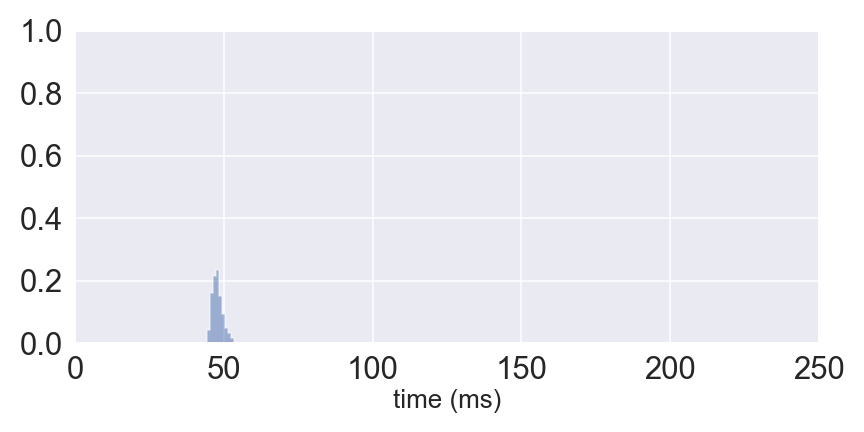
\includegraphics[width=\textwidth,height=.2\textheight,keepaspectratio]{figures/inference_plots/gpu_densenet_inference_time_distribution}}
		\hfill
		\subfloat[B-\gls{densenet}]{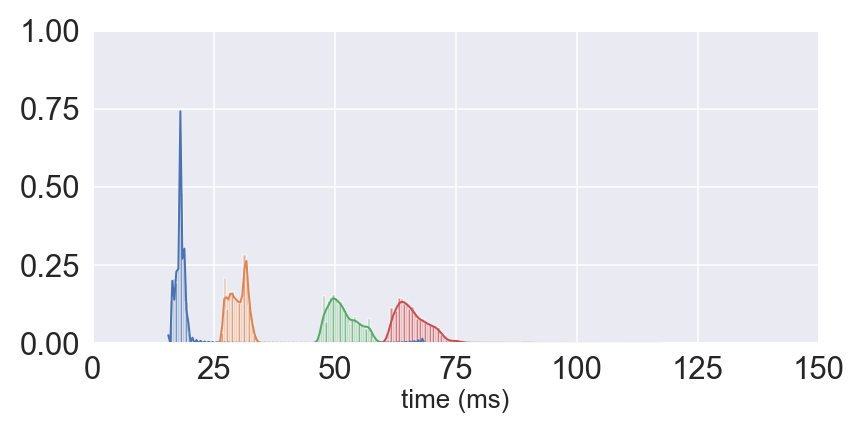
\includegraphics[width=\textwidth,height=.2\textheight,keepaspectratio]{figures/inference_plots/gpu_b-densenet_inference_time_distribution}}
		\hfill
		\subfloat[\gls{msdnet}]{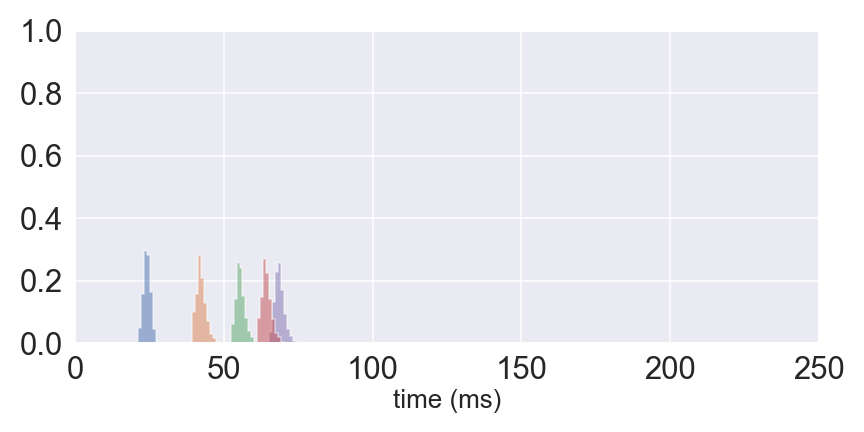
\includegraphics[width=\textwidth,height=.2\textheight,keepaspectratio]{figures/inference_plots/gpu_msdnet_inference_time_distribution}}
	\end{minipage}
	\begin{minipage}{0.33\textwidth}
		\captionsetup[subfigure]{farskip=0pt,captionskip=0pt,justification=centering}
		\centering
		Jetson TX2
		\subfloat[\gls{resnet} ]{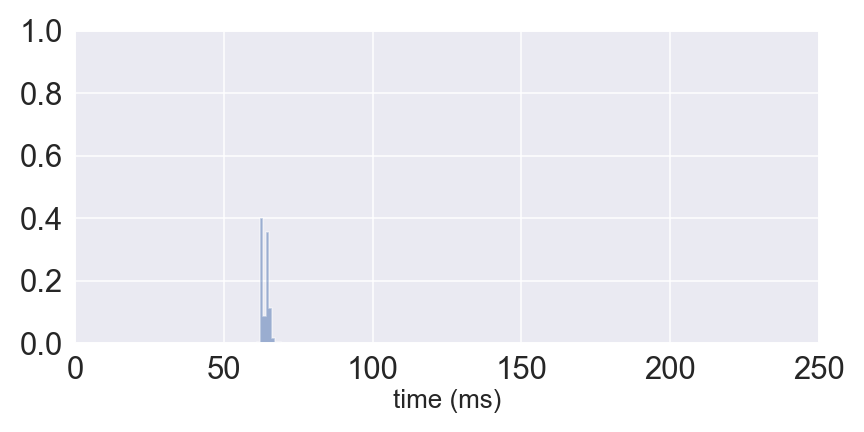
\includegraphics[width=\textwidth,height=.2\textheight,keepaspectratio]{figures/inference_plots/jetson_resnet_inference_time_distribution}}
		\hfill
		\subfloat[B-\gls{resnet}]{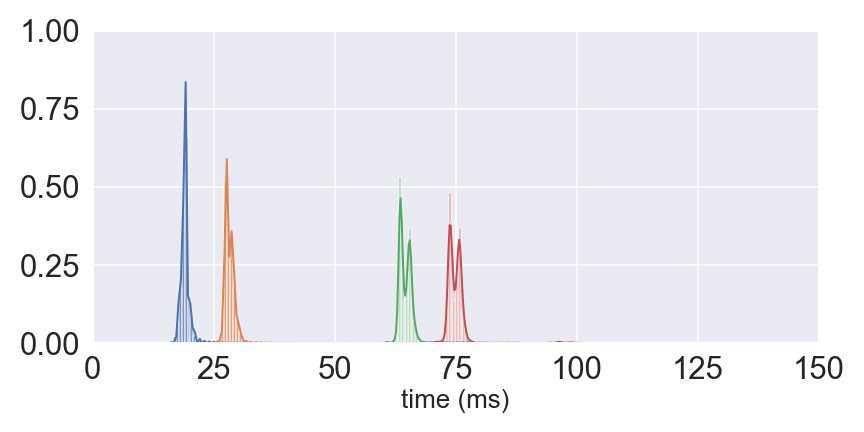
\includegraphics[width=\textwidth,height=.29\textheight,keepaspectratio]{figures/inference_plots/jetson_b-resnet_inference_time_distribution}}
		\hfill
		\subfloat[\gls{densenet} ]{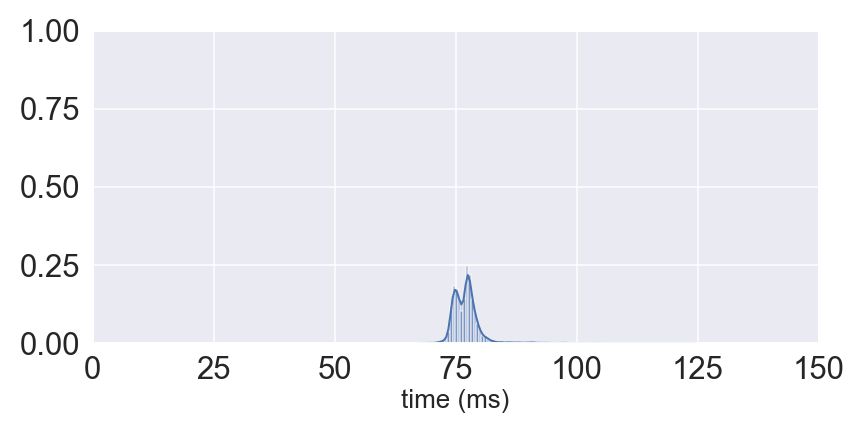
\includegraphics[width=\textwidth,height=.2\textheight,keepaspectratio]{figures/inference_plots/jetson_densenet_inference_time_distribution}}
		\hfill
		\subfloat[B-\gls{densenet}]{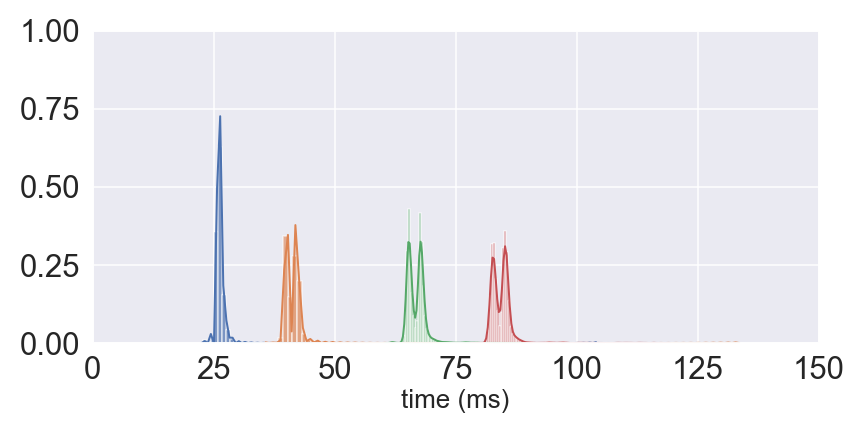
\includegraphics[width=\textwidth,height=.2\textheight,keepaspectratio]{figures/inference_plots/jetson_b-densenet_inference_time_distribution}}
		\hfill
		\subfloat[\gls{msdnet}]{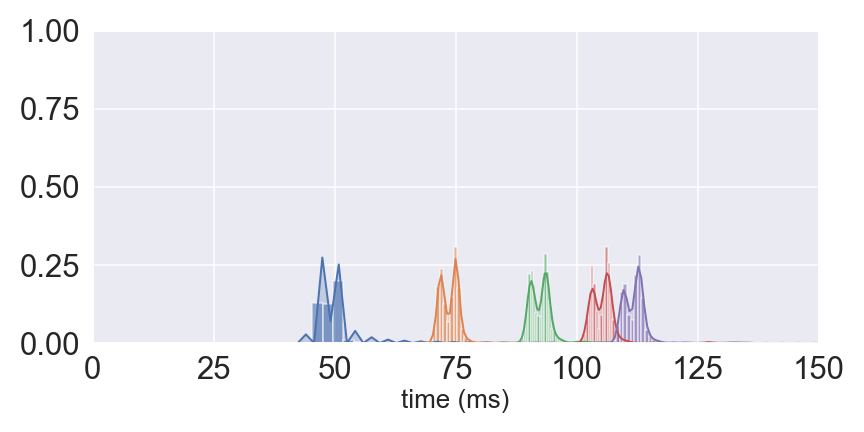
\includegraphics[width=\textwidth,height=.2\textheight,keepaspectratio]{figures/inference_plots/jetson_msdnet_inference_time_distribution}}
	\end{minipage}
	\begin{minipage}{.33\textwidth}
		\captionsetup[subfigure]{farskip=0pt,captionskip=0pt,justification=centering}
		\centering
		Intel NUC
		\subfloat[\gls{resnet} ]{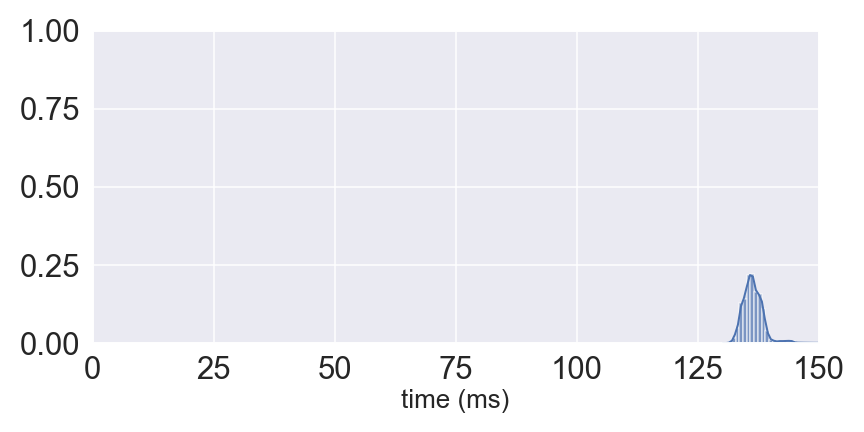
\includegraphics[width=\textwidth,keepaspectratio]{figures/inference_plots/nuc_resnet_inference_time_distribution}}
		\hfill
		\subfloat[B-\gls{resnet}]{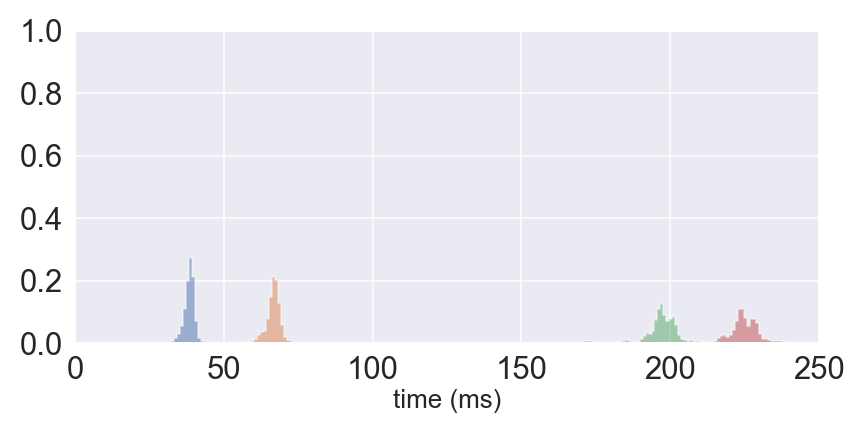
\includegraphics[width=\textwidth,height=.2\textheight,keepaspectratio]{figures/inference_plots/nuc_b-resnet_inference_time_distribution}}
		\hfill
		\subfloat[\gls{densenet} ]{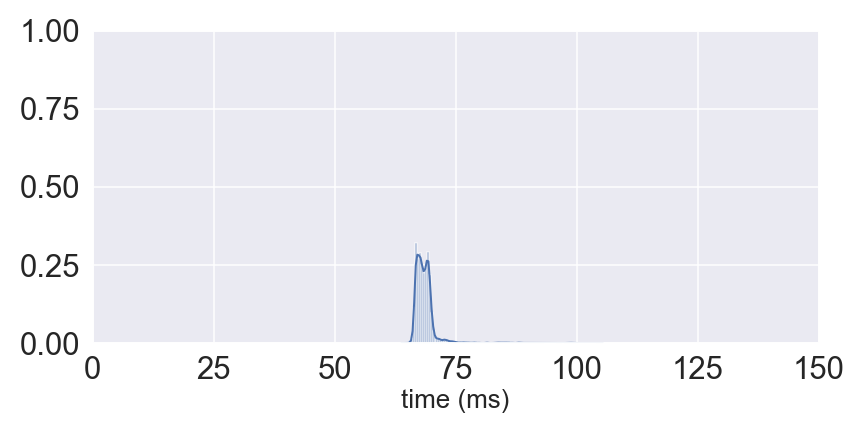
\includegraphics[width=\textwidth,keepaspectratio]{figures/inference_plots/nuc_densenet_inference_time_distribution}}
		\hfill
		\subfloat[B-\gls{densenet}]{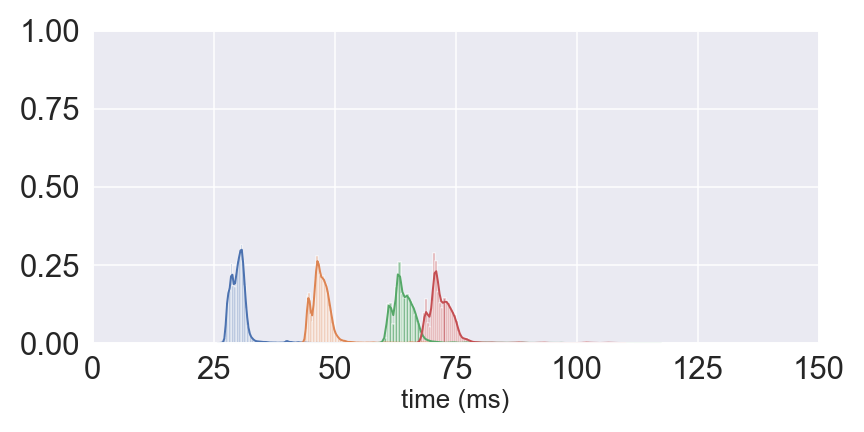
\includegraphics[width=\textwidth,keepaspectratio]{figures/inference_plots/nuc_b-densenet_inference_time_distribution}}
		\hfill
		\subfloat[\gls{msdnet}]{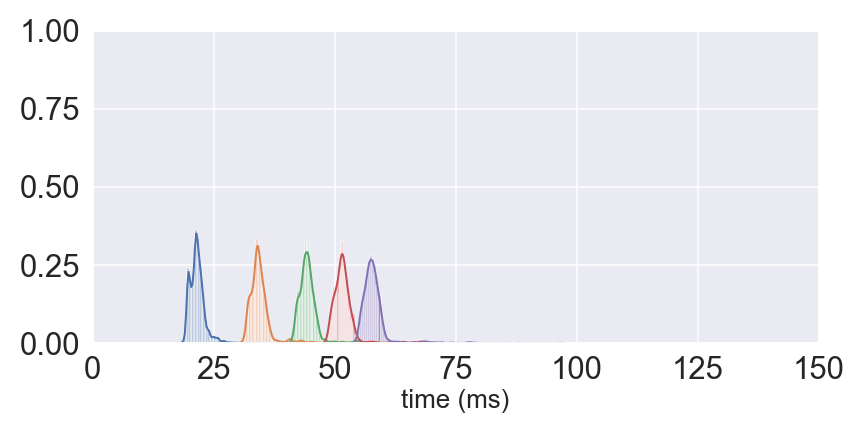
\includegraphics[width=\textwidth,keepaspectratio]{figures/inference_plots/nuc_msdnet_inference_time_distribution}}	
	\end{minipage}
	\caption[Platform Inference Time of \gls{dnn}s]{Inference Time Distribution, left column: GPU Workstation (a-e), center column: Jetson TX2 (f-j), right column NUC (k-o)}
	\label{fig:inference-time-dist}
\end{figure}

Still the challenge remains, how to determine when to let samples exit? It can either be done at random or using the output from the softmax function, which can be interpreted as a confidence metric for the prediction. In the next section we investigate how to allow samples to exit the model prematurely by a study of threshold metrics.


\subsection{Confidence Threshold Analysis}

Selecting threshold is a vital hyper-parameter for the accuracy-latency trade-off of early exiting \gls{branchynet}. If a too high threshold is selected only a few samples can confidently exit the model at an early exit, thus no significant delay improvements may be found. Contrary if too low a threshold is selected a huge delay improvement may be found, however at the cost of overall model accuracy. 

The analysis is theoretical, as the early exiting mechanism is in fact not exploited. All samples are allowed to pass all the way to the end of the network, thus all samples are classified at each exit, where both the prediction and score is logged. The prediction is evaluated against the ground truth and the score against different thresholds. If the score is higher than the threshold the samples is marked as exited. The MiniImageNet100 validation set have been used to evaluate the two threshold metrics; \emph{Confidence Threshold} and \emph{Score-Margin Threshold}. \Cref{fig:resnet_confidence,fig:resnet_score-margin,fig:densenet_confidence,fig:densenet_score-margin,fig:msdnet_confidence,fig:msdnet_score-margin} compares the performance of each exit on all samples. The figures show for each of the three networks under test, a plot of the two thresholds metrics for all exit of the model. The figures shows the frequency of exited samples, that have been correctly classified ({\color{sns-green}green}) and incorrectly classified ({\color{sns-red}red}), and samples that could not be classified with proper confidence given the threshold metric, hence not exited at the exit ({\color{sns-blue}blue}). Along with a plot of the change in accuracy for the exit as the confidence grows ({\color{sns-orange}orange}).  

The aim is to find the metric, that reduces the amount of incorrectly exited samples ({\color{sns-red}red}). Whenever samples are exited incorrectly, the overall accuracy of the models are reduced, if it could have been correctly classifed at later exit. The growing frequency of correctly exited samples ({\color{sns-green}green}) at later exits shows exactly this. As the threshold requirements are raised, it results in a higher accuracy for the exit, as the ratio between correctly exited and incorrectly exited grows. 

Generally \emph{score-margin} has more desirable traits, as less samples are incorrectly exited ({\color{sns-red}red}), at the expense of additional samples not exited ({\color{sns-blue}blue}). \emph{Score-margin} is thus slower, but also more accurate, as fewer samples are incorrectly exited. The results matches \cite{park_big/little_2015}, which show a stronger correlation between \emph{score-margin} and accuracy, than confidence score and accuracy. Henceforth the \emph{score-margin threshold} are used.

Comparing the three models we can see the impact of densely connected layer of B-\gls{densenet} and \gls{msdnet}. The two model are able to obtain higher scores at early exits, thus accurately exiting more samples prematurely. B-\gls{resnet} on the other hand are able to achieve higher end accuracy, ass we did show in the previous section \ref{sec:early-exit-analysis}. The theoretical analysis is followed up by a practical test, where samples are exited if the threshold is passed. The test evaluates the threshold impact on accuracy and latency. 

\newcounter{imagenumber}
\begin{minipage}{\textwidth}
\begin{figure}
	\centering
	\paragraph{B-ResNet}
	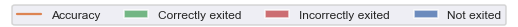
\includegraphics[width=\linewidth]{figures/threshold_plots/threshold_analysis_legend}
\end{figure}

\begin{minipage}{0.5\textwidth}
	\begin{figure}
		\captionsetup[subfloat]{farskip=1pt,captionskip=1pt, justification=centering}
		\centering
		\forloop{imagenumber}{0}{\value{imagenumber} < 4}{
			
			\subfloat[Exit-\arabic{imagenumber}\label{fig:confidence_resnet_exit_\arabic{imagenumber}}]{\includegraphics[width=.9\linewidth]{figures/threshold_plots/threshold_analysis_b-resnet_confidence_\arabic{imagenumber}}}
			\hfill
		}
		\caption[ResNet Confidence Threshold]{Confidence Threshold}
		\label{fig:resnet_confidence}
	\end{figure}
\end{minipage}
\begin{minipage}{0.5\textwidth}
	\begin{figure}
		\captionsetup[subfloat]{farskip=1pt,captionskip=1pt, justification=centering}
		\centering
		\forloop{imagenumber}{0}{\value{imagenumber} < 4}{
			
			\subfloat[Exit-\arabic{imagenumber}\label{fig:score-margin_resnet_exit_\arabic{imagenumber}}]{\includegraphics[width=.9\linewidth]{figures/threshold_plots/threshold_analysis_b-resnet_score-margin_\arabic{imagenumber}}}
			\hfill
		}
		\caption[ResNet Score-margin Threshold]{Score-margin Threshold}
		\label{fig:resnet_score-margin}
	\end{figure}
\end{minipage}
\end{minipage}

\begin{minipage}{\textwidth}
	\begin{figure}
		\centering
		\paragraph{B-DenseNet}
	\end{figure}
	\begin{minipage}{0.5\textwidth}
		\begin{figure}
			\captionsetup[subfloat]{farskip=1pt,captionskip=1pt, justification=centering}
			\centering
			\forloop{imagenumber}{0}{\value{imagenumber} < 4}{
				
				\subfloat[Exit-\arabic{imagenumber}\label{fig:confidence_dense_exit_\arabic{imagenumber}}]{\includegraphics[width=.9\linewidth]{figures/threshold_plots/threshold_analysis_b-densenet_confidence_\arabic{imagenumber}}}
				\hfill
			}
			\caption[DenseNet Confidence Threshold]{Confidence Threshold}
			\label{fig:densenet_confidence}
		\end{figure}
	\end{minipage}
	\begin{minipage}{0.5\textwidth}
		\begin{figure}
			\captionsetup[subfloat]{farskip=1pt,captionskip=1pt, justification=centering}
			\centering
			\forloop{imagenumber}{0}{\value{imagenumber} < 4}{
				
				\subfloat[Exit-\arabic{imagenumber}\label{fig:score-dense_resnet_exit_\arabic{imagenumber}}]{\includegraphics[width=.9\linewidth]{figures/threshold_plots/threshold_analysis_b-densenet_score-margin_\arabic{imagenumber}}}
				\hfill
			}
			\caption[DenseNet Score-margin Threshold]{Score-margin Threshold}
			\label{fig:densenet_score-margin}
		\end{figure}
	\end{minipage}
\end{minipage}

\noindent\makebox[\textwidth][c]{\begin{minipage}{0.9\textwidth}
	\begingroup
	\leftskip=0cm plus 0.5fil \rightskip=0cm plus -0.5fil
	\parfillskip=0cm plus 1fil
	\paragraph{MSDNet}\par
	\endgroup
	
	\begin{minipage}{0.5\textwidth}
		\begin{figure}
			\captionsetup[subfloat]{farskip=0pt,captionskip=0pt, justification=centering}
			\centering
			\forloop{imagenumber}{0}{\value{imagenumber} < 5}{
				
				\subfloat[Exit-\arabic{imagenumber}\label{fig:confidence_msd_exit_\arabic{imagenumber}}]{\includegraphics[width=.9\linewidth]{figures/threshold_plots/threshold_analysis_msdnet_confidence_\arabic{imagenumber}}}
				\hfill
			}
			\caption[MSDNet Confidence Threshold]{Confidence Threshold}
			\label{fig:msdnet_confidence}
		\end{figure}
	\end{minipage}
	\begin{minipage}{0.5\textwidth}
		\begin{figure}
			\captionsetup[subfloat]{farskip=1pt,captionskip=1pt, justification=centering}
			\centering
			\forloop{imagenumber}{0}{\value{imagenumber} < 5}{
				
				\subfloat[Exit-\arabic{imagenumber}\label{fig:score-msdnet_exit_\arabic{imagenumber}}]{\includegraphics[width=.9\linewidth]{figures/threshold_plots/threshold_analysis_msdnet_score-margin_\arabic{imagenumber}}}
				\hfill
			}
			\caption[MSDNet Score-margin Threshold]{Score-margin Threshold}
			\label{fig:msdnet_score-margin}
		\end{figure}
	\end{minipage}
\end{minipage}}

\subsubsection{Practical Threshold Exiting}

We construct a test, where we use our three models, B-\gls{resnet}, B-\gls{densenet} and \gls{msdnet}, to evaluate early exiting capabilities. In this test a sample is exited when a threshold is passed, thus no additional prediction are tried for the sample. If a samples reaches the last exit, it is classified irregardless of threshold being passed or not.


\begin{figure}
	\centering
	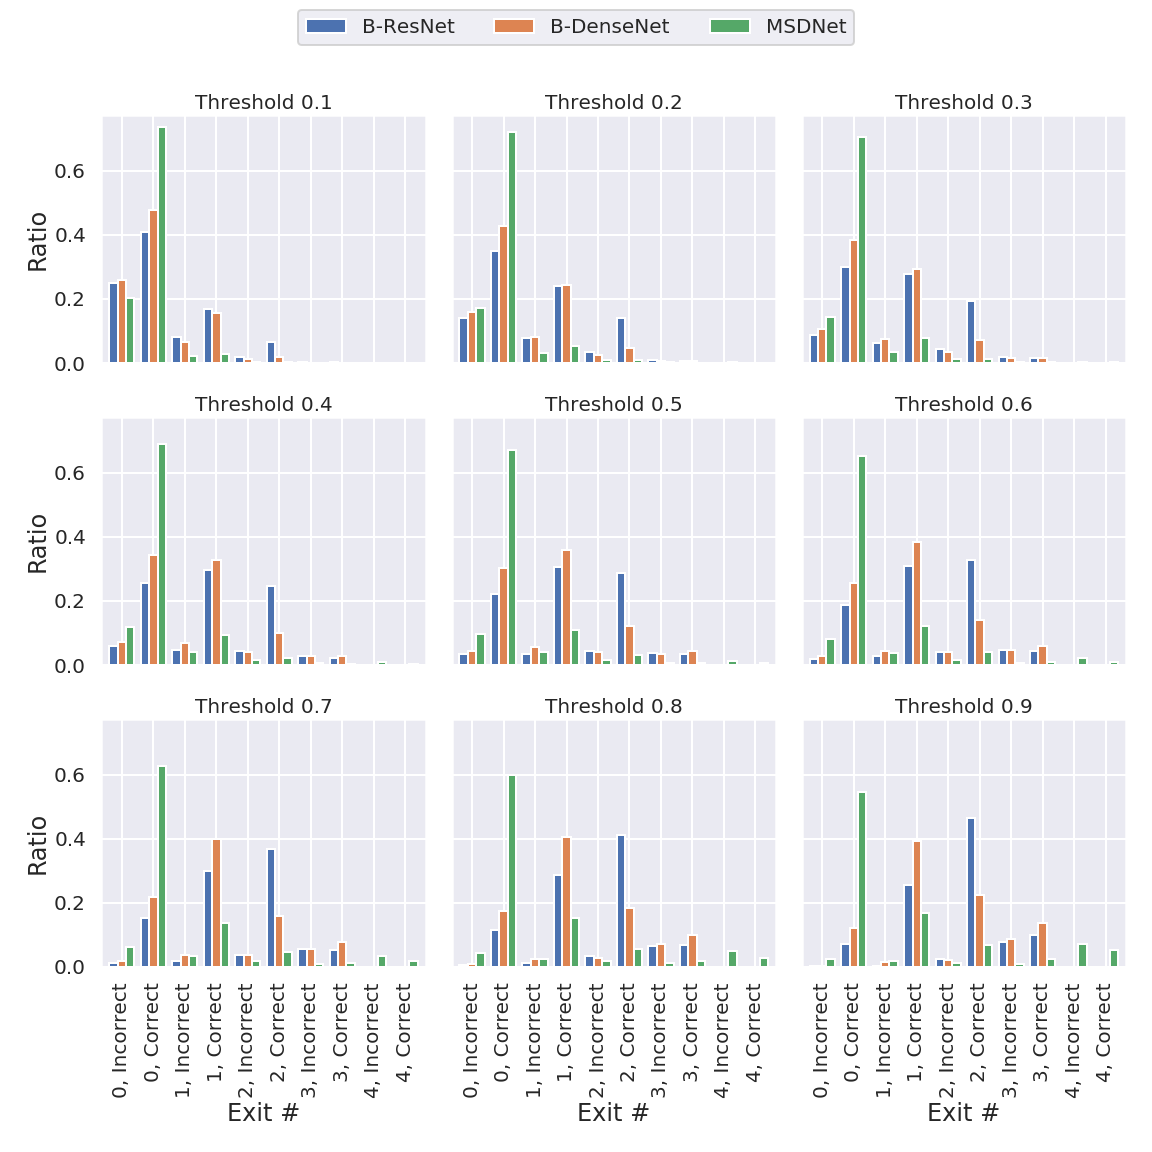
\includegraphics[width=\linewidth]{figures/threshold_plots/inference_threshold_test}
	\caption{Score-Margin Exiting}
	\label{fig:inferencethresholdtest}
\end{figure}

\begin{minipage}{\linewidth}
	\begin{figure}
		\captionsetup[subfloat]{justification=centering, captionskip=0pt, farskip=0pt}
		\centering
		
\includegraphics[width=.5\linewidth]{figures/inference_plots/model_bar_legend}
	\end{figure}
	\begin{figure}
		\captionsetup[subfloat]{justification=centering, captionskip=0pt, farskip=1pt}
		\centering
		\subfloat[$T= 0.1$\label{fig:model-threshold_comparison_t_1}]{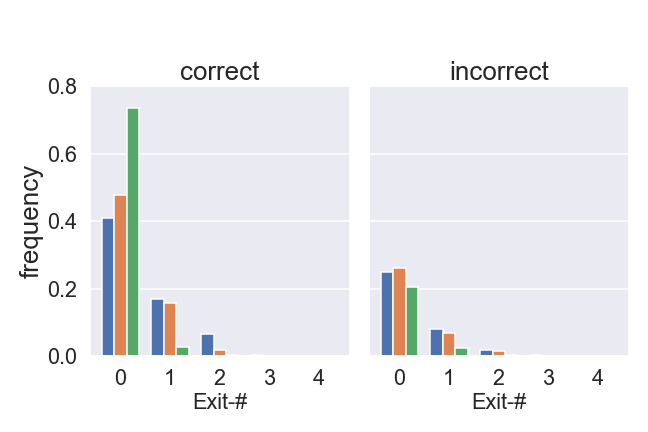
\includegraphics[width=.33\linewidth]{figures/inference_plots/model_comparison_1}}
		\hfill
		\subfloat[$T= 0.2$\label{fig:model-threshold_comparison_t_2}]{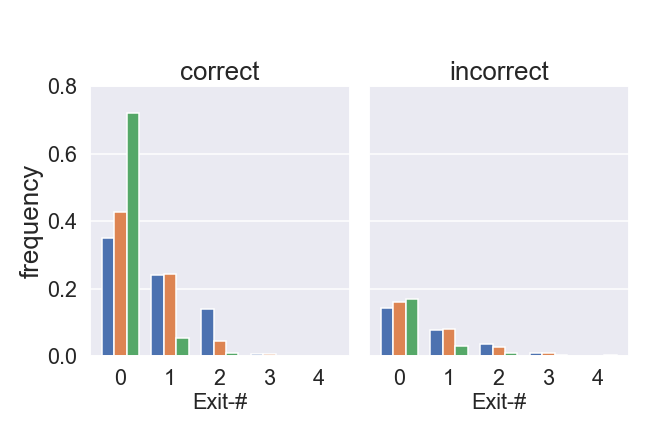
\includegraphics[width=.33\linewidth]{figures/inference_plots/model_comparison_2}}
		\hfill
		\subfloat[$T= 0.3$\label{fig:model-threshold_comparison_t_3}]{\includegraphics[width=.33\linewidth]{figures/inference_plots/model_comparison_3}}
		\hfill
		\subfloat[$T= 0.4$\label{fig:model-threshold_comparison_t_4}]{\includegraphics[width=.33\linewidth]{figures/inference_plots/model_comparison_4}}
		\hfill
		\subfloat[$T= 0.5$\label{fig:model-threshold_comparison_t_5}]{\includegraphics[width=.33\linewidth]{figures/inference_plots/model_comparison_5}}
		\hfill
		\subfloat[$T= 0.6$\label{fig:model-threshold_comparison_t_6}]{\includegraphics[width=.33\linewidth]{figures/inference_plots/model_comparison_6}}
		\hfill
		\subfloat[$T= 0.7$\label{fig:model-threshold_comparison_t_7}]{\includegraphics[width=.33\linewidth]{figures/inference_plots/model_comparison_7}}
		\hfill
		\subfloat[$T= 0.8$\label{fig:model-threshold_comparison_t_8}]{\includegraphics[width=.33\linewidth]{figures/inference_plots/model_comparison_8}}
		\hfill
		\subfloat[$T= 0.9$\label{fig:model-threshold_comparison_t_9}]{\includegraphics[width=.33\linewidth]{figures/inference_plots/model_comparison_9}}
		
		\caption[Model comparison of early exit capabilities]{Model comparison of early exit capabilities}
		\label{fig:model_threshold_comparison}
	\end{figure}

\end{minipage}

Figure \ref{fig:inferencethresholdtest} the exiting capabilities for the model at different \emph{score-margin threshold}. The frequency of correct and incorrect prediction are plotted for each exit. For each model the bars sum to one, equivalent to all samples of the test. The figure shows, that less samples are incorrect classified, as we select a higher threshold and thus forcing the model to use later exits. B-\gls{densenet} and especially \gls{msdnet}  designed for early-exiting, are able to more frequently exit samples at early exits even at high thresholds values. Given this insight we use timings from the test to evaluate threshold impact on the accuracy-latency trade-off.

%\subsubsection{Accuracy-Latency Trade-Off Analysis}

Figure \ref{fig:threshold-acc-lat-trade-off} show the inference accuracy and time on the three different platforms. The result clearly exemplifies the accuracy-latency trade-off imposed by early exiting. As we raise our requirements for confidence, we improve the model accuracy, but more time is used, as later exits are required to reach the level of confidence. The conventional models are clearly more accurate, however also expectantly slower, than their more flexible exiting counterpart. B-\gls{densenet} benefits more from early exiting, when a threshold of 0.9 is chosen, it gives up 4 percentage point in accuracy and reducing inference latency by 29 \%. The B-\gls{resnet} have about the same compromise in terms of accuracy, however only a reduction of 18 \% inference latency. B-\gls{resnet} still perform better in terms of both accuracy and inference time on the \gls{gpu}-enabled devices. 

As previously shown the models using densely connected layers are able to exit more samples early.

\begin{figure}
  	\captionsetup[subfigure]{justification=centering,farskip=0pt,captionskip=0pt}
  	\centering
  	\includegraphics[width=.5\linewidth]{figures/threshold_plots/inference_legend}
  	\subfloat[GPU Workstation\label{fig:early_exit_vs_conv}]{\includegraphics[width=\textwidth,height=.29\textheight,keepaspectratio]{figures/threshold_plots/gpu_inference}}
  	\hfill
	\subfloat[Jetson TX2\label{fig:jetson-early_exit_vs_conv}]{\includegraphics[width=\textwidth,height=.29\textheight,keepaspectratio]{figures/threshold_plots/jetson_inference}}
	\hfill
	\subfloat[NUC\label{fig:nuc-early_exit_vs_conv}]{\includegraphics[width=\textwidth,height=.29\textheight,keepaspectratio]{figures/threshold_plots/nuc_inference}}
	\caption[Threshold Accuracy-Latency Trade-off]{Threshold Accuracy-Latency Trade-off on \protect\subref{fig:early_exit_vs_conv} GPU Workstation, \protect\subref{fig:jetson-early_exit_vs_conv} Jetson TX2 and \protect\subref{fig:nuc-early_exit_vs_conv} NUC }
	\label{fig:threshold-acc-lat-trade-off}
\end{figure}


%  \begin{figure}
%	\captionsetup[subfigure]{justification=centering}
%	\centering
%	\subfloat[Jetson TX2 fine-grained\label{fig:jetson-fingrained}]{\includegraphics[width=\linewidth]{figures/threshold_plots/jetson_inference_finegrained}}
%	\caption[]{}
%\end{figure}

\subsection{Delay Threshold Analysis}

For time-budgeted applications, where a classification must be derived within a timed threshold. We wish to maximize the accuracy subject to this time constraint. Figure \ref{fig:time-threshold} show the model accuracy under different time constraints and on different platforms.

How to choose threshold?
If given a time threshold, what accuracy are we then able to achieve? 

\begin{figure}
	\captionsetup[subfigure]{justification=centering}
	\centering
	\subfloat[GPU Workstation]{\includegraphics[width=\textwidth,height=.29\textheight,keepaspectratio]{figures/threshold_plots/time_threshold_pc}}
	\hfill
	\subfloat[Jetson TX2]{\includegraphics[width=\textwidth,height=.29\textheight,keepaspectratio]{figures/threshold_plots/time_threshold_jetson}}
	\hfill
	\subfloat[NUC]{\includegraphics[width=\textwidth,height=.29\textheight,keepaspectratio]{figures/threshold_plots/time_threshold_nuc}}
	\caption[Time Threshold]{Time Threshold}
	\label{fig:time-threshold}
\end{figure}

From figure \ref{fig:inference-time-dist} we know the inference time distribution for each exit on different hardwares. Given a time constraint, we can selective choose the exit with the best chance to provide a prediction within a certain time frame, similar to Edgent \cite{li_edge_2018}. The difference at first is we only focus on on-device or on-edge execution  with no collaboration, hence we do not need a regression model of the per layer execution of the \gls{dnn}. For device-only execution our only concern is the inference time on the specific hardware, a simple selection would be the exit with the largest inference time mean within the time constraint, as accuracy is monotically increasing over available time.
\begin{maxi*}
			{}{Reliabilty\sim\tau_{computation}}
	{}{}
	\addConstraint{\tau_{computation}}{\leq T}
\end{maxi*}
 In an edge-offloading scenario we must consider communication latency. If the available networking conditions are good a later exit can be chosen to improve the reliability, however in scenarios, where networking conditions are poor an earlier exit must be chosen to meet latency requirements. 
 \begin{maxi*}
 	{}{Reliabilty\sim\tau_{computation}}
 	{}{}
 	\addConstraint{(\tau_{computation}+\tau_{communication})}{\leq T}
 \end{maxi*}
The selection of exit is based on distributions of inference time, this introduces some uncertainty, as not all samples might be able to meet the latency requirement, this can be caused be derivation in compute time, congestions in the network latency or server workload. One key feature of early exiting is the ability to obtain intermediate predictions, this allow for parallel execution while offloading. The end-device might only be able to reach an early exit within the time frame, where edge server reaches a later one. However, unexpectedly no reply is received by the end-device within the time frame, then the application can use the local obtained prediction from an earlier exit. 

Or a collaborative scheme might be used, where the end-device locally processes the algorithm up to an early exit and obtains a prediction, then it offload the rest of the execution in a cascaded manner for remote execution, still if no reply is received by the end-device within the time frame a locally obtained prediction is available albeit less reliable than if the remote prediction would have arrived in time. Multiple early exits allows for successively sending back increasingly confident and reliable predictions, at a small overhead communication, the last received prediction would then be used by the application.